\documentclass[12pt]{article}
\usepackage[utf8]{inputenc}
\usepackage[T1]{fontenc}
\usepackage[top=0.60in, bottom=0.80in, left=0.60in, right=0.60in]{geometry}
\usepackage{graphicx}
\usepackage{siunitx}
\usepackage{listings}

\newcommand{\Msun}{\mathrm{M_{\odot}}}
\newcommand{\Rsun}{\mathrm{R_{\odot}}}
\newcommand{\MWD}{M_{\mathrm{WD}}}
\newcommand{\Mstar}{M_{\star}}
\newcommand{\alphace}{\alpha_{\mathrm{CE}}}
\newcommand{\alphath}{\alpha_{\mathrm{th}}}
\newcommand{\alpharec}{\alpha_{\mathrm{rec}}}
\newcommand{\Ebind}{E_{\mathrm{bind}}}
\newcommand{\Egrav}{E_{\mathrm{grav}}}
\newcommand{\Eint}{E_{\mathrm{int}}}
\newcommand{\Eth}{E_{\mathrm{th}}}
\newcommand{\Erec}{E_{\mathrm{rec}}}
\newcommand{\Porb}{P_{\mathrm{orb}}}
\newcommand{\au}{\, \mathrm{au}}

\title{Wide Post-Mass Transfer White-Dwarf Binaries}
\author{Runqiu Ye}
\date{June, 2024}

\begin{document}

\maketitle

\section{Introduction}
Common envelope (CE) is the outcome of unstable mass transfer. During CE, both stars orbit inside an envelope and spiral inward. If the energy liberated in this process is enough to eject the CE, then the result of CE process is a close binary. If, on the contrary, the liberated energy is not enough to eject the envelope, then the result of the process is a merger. In observation results, a number of WD+MS binaries are wider than expected, and CE is expected to be the main channel to form these white dwarf binaries \cite{yamaguchi_hi, yamaguchi_lo}. In the MESA model utilized by \cite{yamaguchi_hi, yamaguchi_lo}, wide post-CE WD+MS binaries can be formed in a certain range of initial separation with only gravitational and internal energy included in the calculation. 

In this paper, we are going to explore the formation of these wide post-mass transfer WD+MS binaries with COSMIC model. We perform COSMIC simulation on both individual binary star systems and sampled population to explore the formation of WD+MS binaries under different conditions. In section 2, we are going to investigate formation of individual wide WD+MS binaries through CE for a variety of variables, including initial mass, initial separation, common envelope efficiency, and the energy budget of the CE. In section 3, we are going to explore the formation of individual wide WD+MS binaries through stable mass transfer. In section 4, we will research on how different COSMIC model affect simulation results of a sample population of binary star systems, and how the formation of post WD+MS binaries depends on various parameters.

\section{Common Envelope}

As argued in \cite{yamaguchi_hi,yamaguchi_lo}, unstable mass transfer is expect to be the main channel to form wide WD+MS binaries. In the MESA model, wide post-CE WD+MS binaries can be formed in certain range of initial separation. We hope to explore similar models in COSMIC.

In \cite{yamaguchi_hi}, the lower limit of WD mass $M_{\mathrm{MD, min}}$ in the observational sample is calculated to be $1.244\Msun \sim 1.418\Msun$. The corresponding mass of MS progenitor is expected to be in the range of $6 \sim 9 \Msun$, and the companion mass has median around $1\Msun$. In \cite{yamaguchi_lo}, the WD mass in the Gaia sample ranges from $0.5\Msun$ to $0.8\Msun$, which corresponds to progenitor mass of $1 \Msun$ to $3 \Msun$. The companions mass $\Mstar$ has a median of $0.85 \Msun$. Hence, we consider high mass systems using a $7\Msun + 1\Msun$ binary and low mass systems using a $1.5\Msun + 0.85\Msun$

\subsection{High mass systems ($7\Msun + 1\Msun$)}
In \cite{yamaguchi_hi}, the authors discussed currently observed wide post-mass transfer binary star systems. The MS progenitor of the WD star is expected to be in the range of $6 \sim 9 \Msun$. Therefore, MESA model of a $7\Msun$ star is run, and the evolution up to AGB is followed. After that, the change of separation through common envelope is calculated with
\[
E_{\mathrm{bind}} = \alphace \left(-\frac{G\MWD \Mstar}{2a_f}+\frac{GM_i \Mstar}{2a_i}\right).
\]
The binding energy on LHS is calculated as
\[
E_{\mathrm{bind}} = E_{\mathrm{grav}} + E_{\mathrm{int}} = \int_{M_{\mathrm{core}}}^{M_{\mathrm{tot}}} -\frac{Gm}{r(m)} + U(m) dm
\]
or
\[
	E_{\mathrm{bind}} = E_{\mathrm{grav}} + \alphath E_{\mathrm{th}} + \alpharec E_{\mathrm{rec}}.
\]
The results is presented in Figure \ref{yam_hi}, and we want to compare how this energy budget matches with the binding energy in COSMIC. Usually, the binding energy of the common envelope can be included in a structure parameter $\lambda$ such that 

\begin{equation}
	\Ebind = \frac{G M_i M_{\mathrm{env}}}{\lambda R_i}.   
	\label{ebind}
\end{equation}

This $\lambda$ is represented in COSMIC as the \verb|lambdaf| flag in \verb|BSEDict|. Hence, we want to calculate the effective $\lambda$ in COSMIC that matches these binding energy models in MESA.

\begin{figure}
    \centering
    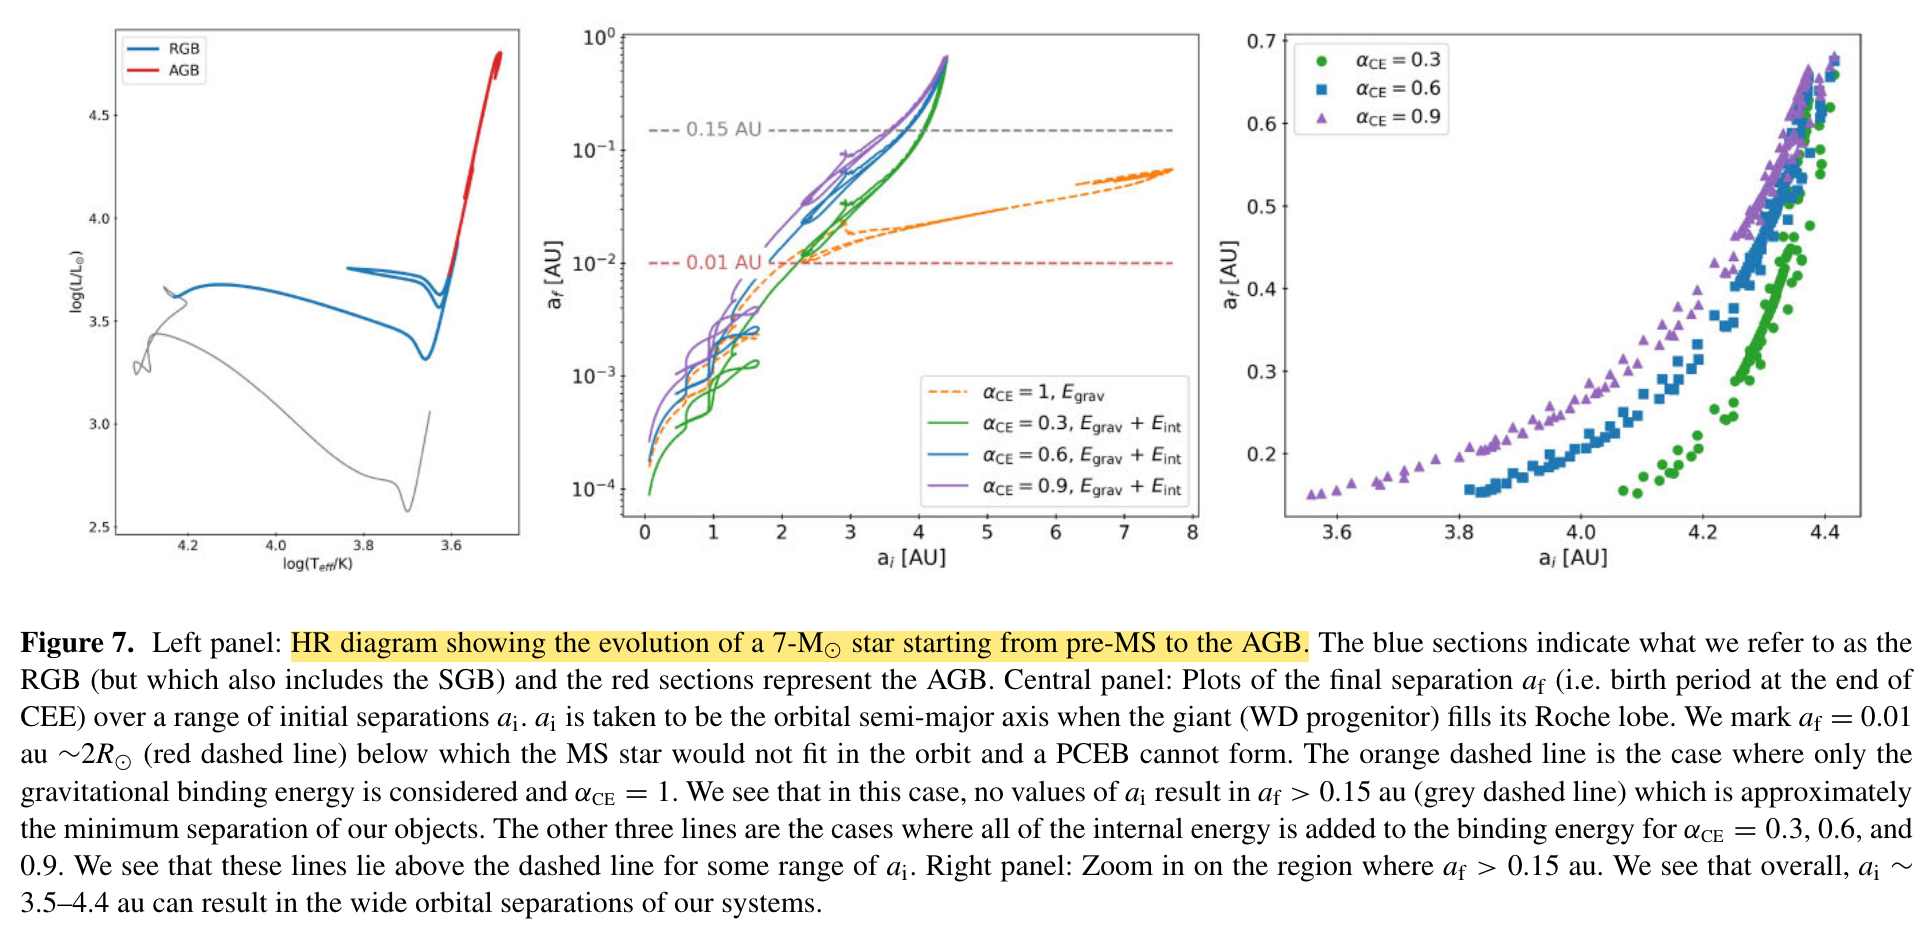
\includegraphics[width=\linewidth]{yamaguchi-7+1.png}
    \caption{Results of how final separation $a_f$ after common envelope depends on initial separation $a_i$ for different common envelope efficiencies and energy budgets in \cite{yamaguchi_hi}.}
    \label{yam_hi}
\end{figure}

\subsubsection{Methods and results}
To compare model in COSMIC with model in MESA, we run COSMIC binary simulation of a $7\Msun + 1\Msun$ system. We want to see how the final separation $a_f$ depends on the initial separation $a_i$ and the common envelope parameter $\lambda$. Hence, we vary the initial separation in range $2 \sim 8 \au$ and the common envelope flag \verb|lambdaf| in range $0 \sim -100$, which corresponds to $0 \sim 100$ for $\lambda$. Also, we run these parameters with four different common envelope efficiencies — $\alphace = 1$, $\alphace = 0.9$, $\alphace = 0.6$, and $\alphace = 0.3$.

After simulation is finished, we select the timestep that the system finished common envelope for the first time (\verb|evol_type = 8|). At this moment, if the system is a WD+MS system, we record their separation as the final separation $a_f$. Otherwise, we set $a_f = 0$ and consider this initial condition unable to produce a WD+MS system.

We write the resulting final separations into \verb|csv| files and create four heat maps for the four different common envelope efficiencies, as shown in Figure \ref{res_hi}.

\begin{figure}
    \centering
    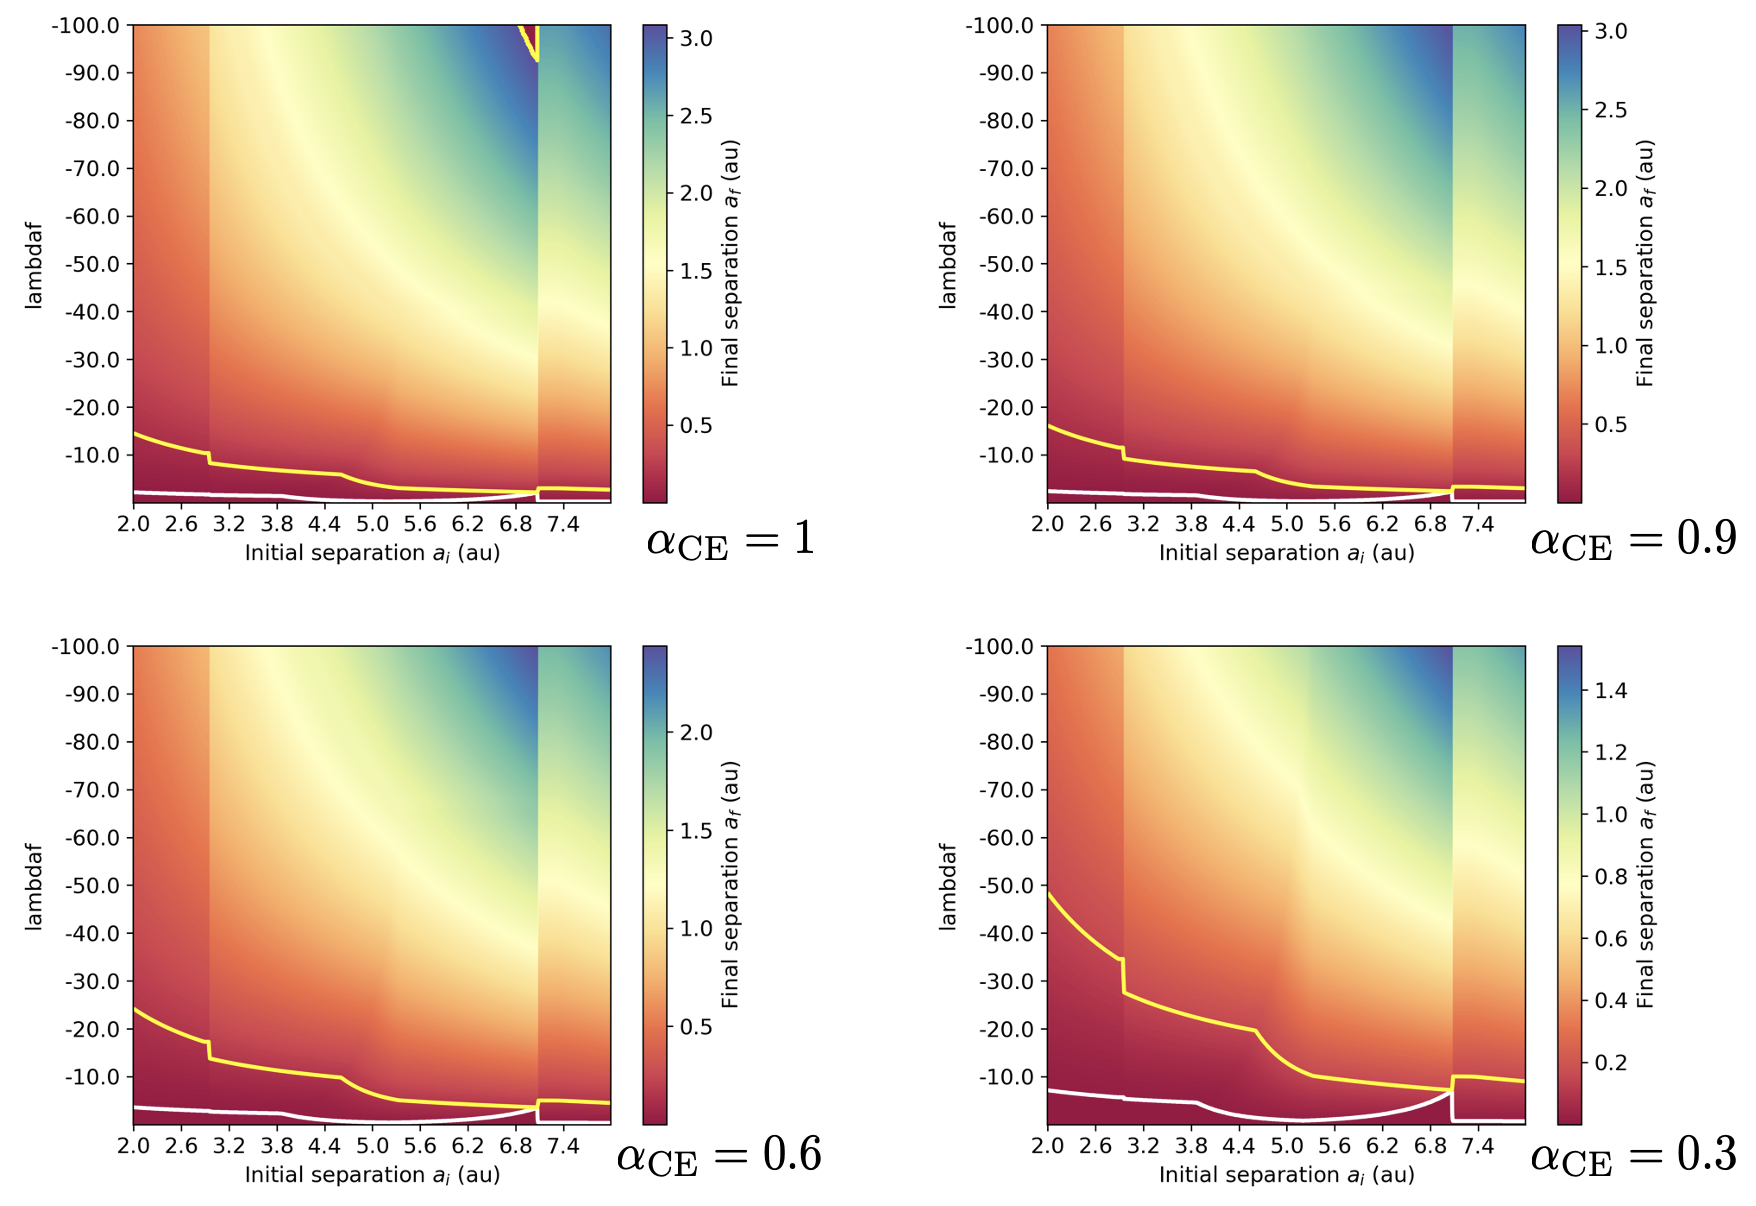
\includegraphics[width=0.9\linewidth]{7+1results.png}
    \caption{COSMIC results of how final separation $a_f$ depends on initial separation $a_i$ and common envelope flag "lambdaf" for different common envelope efficiencies $\alphace$, where the black and red contour corresponds to $0.01 \au$ and $0.15 \au$ as in Figure \ref{yam_hi} respectively. Outside the black contour no desired system forms.}
    \label{res_hi}
\end{figure}
% =========================== Current Position ===========================
\subsubsection{Discussions}
Taking a closer look as the heatmap in Figure \ref{res_hi}, we notice a few interesting points. 

First of all, as $\alphace$ decreases, the final separation decreases in general. This is expected and can be clearly derived from the formula. Qualitatively, more energy from the orbit is needed to eject the envelope for low $\alphace$, so the resulting $a_f$ is smaller. 

In addition, it is worth noting that most of these systems experience two mass transfer phases in COSMIC before reaching WD+MS. That is, two common evenlope phases take places, between which there's a period of time. For some cases \verb|kstar_1| changes during this period.

Also notice that the final separation $a_f$ jumps obviously at about $2.9 \au$, and $7.1 \au$, which can be clearly seen from the graph. After investigating the \verb|bpp| array of these simulations, we find out the jump at about $2.9 \au$ and $7.1 \au$ is likely due to the difference of \verb|kstar_1| at the start of RLOF. For $a_i < 2.9 \au$, RLOF starts when \verb|kstar_1 = 3| (First Giant Branch, GB). For $a_i = 2.9 \au$, RLOF starts when \verb|kstar_1 = 4| (Core Helium Burning, CHeB). For $2.9 \au < a_i < 7.1 \au$, RLOF starts when \verb|kstar_1 = 5|, (Early AGB, E-AGB). For $a_i > 7.1 \au$, RLOF starts when \verb|kstar_1 = 6|, (thermal-pulse AGB, TP-AGB). 

\begin{figure}
    \centering
    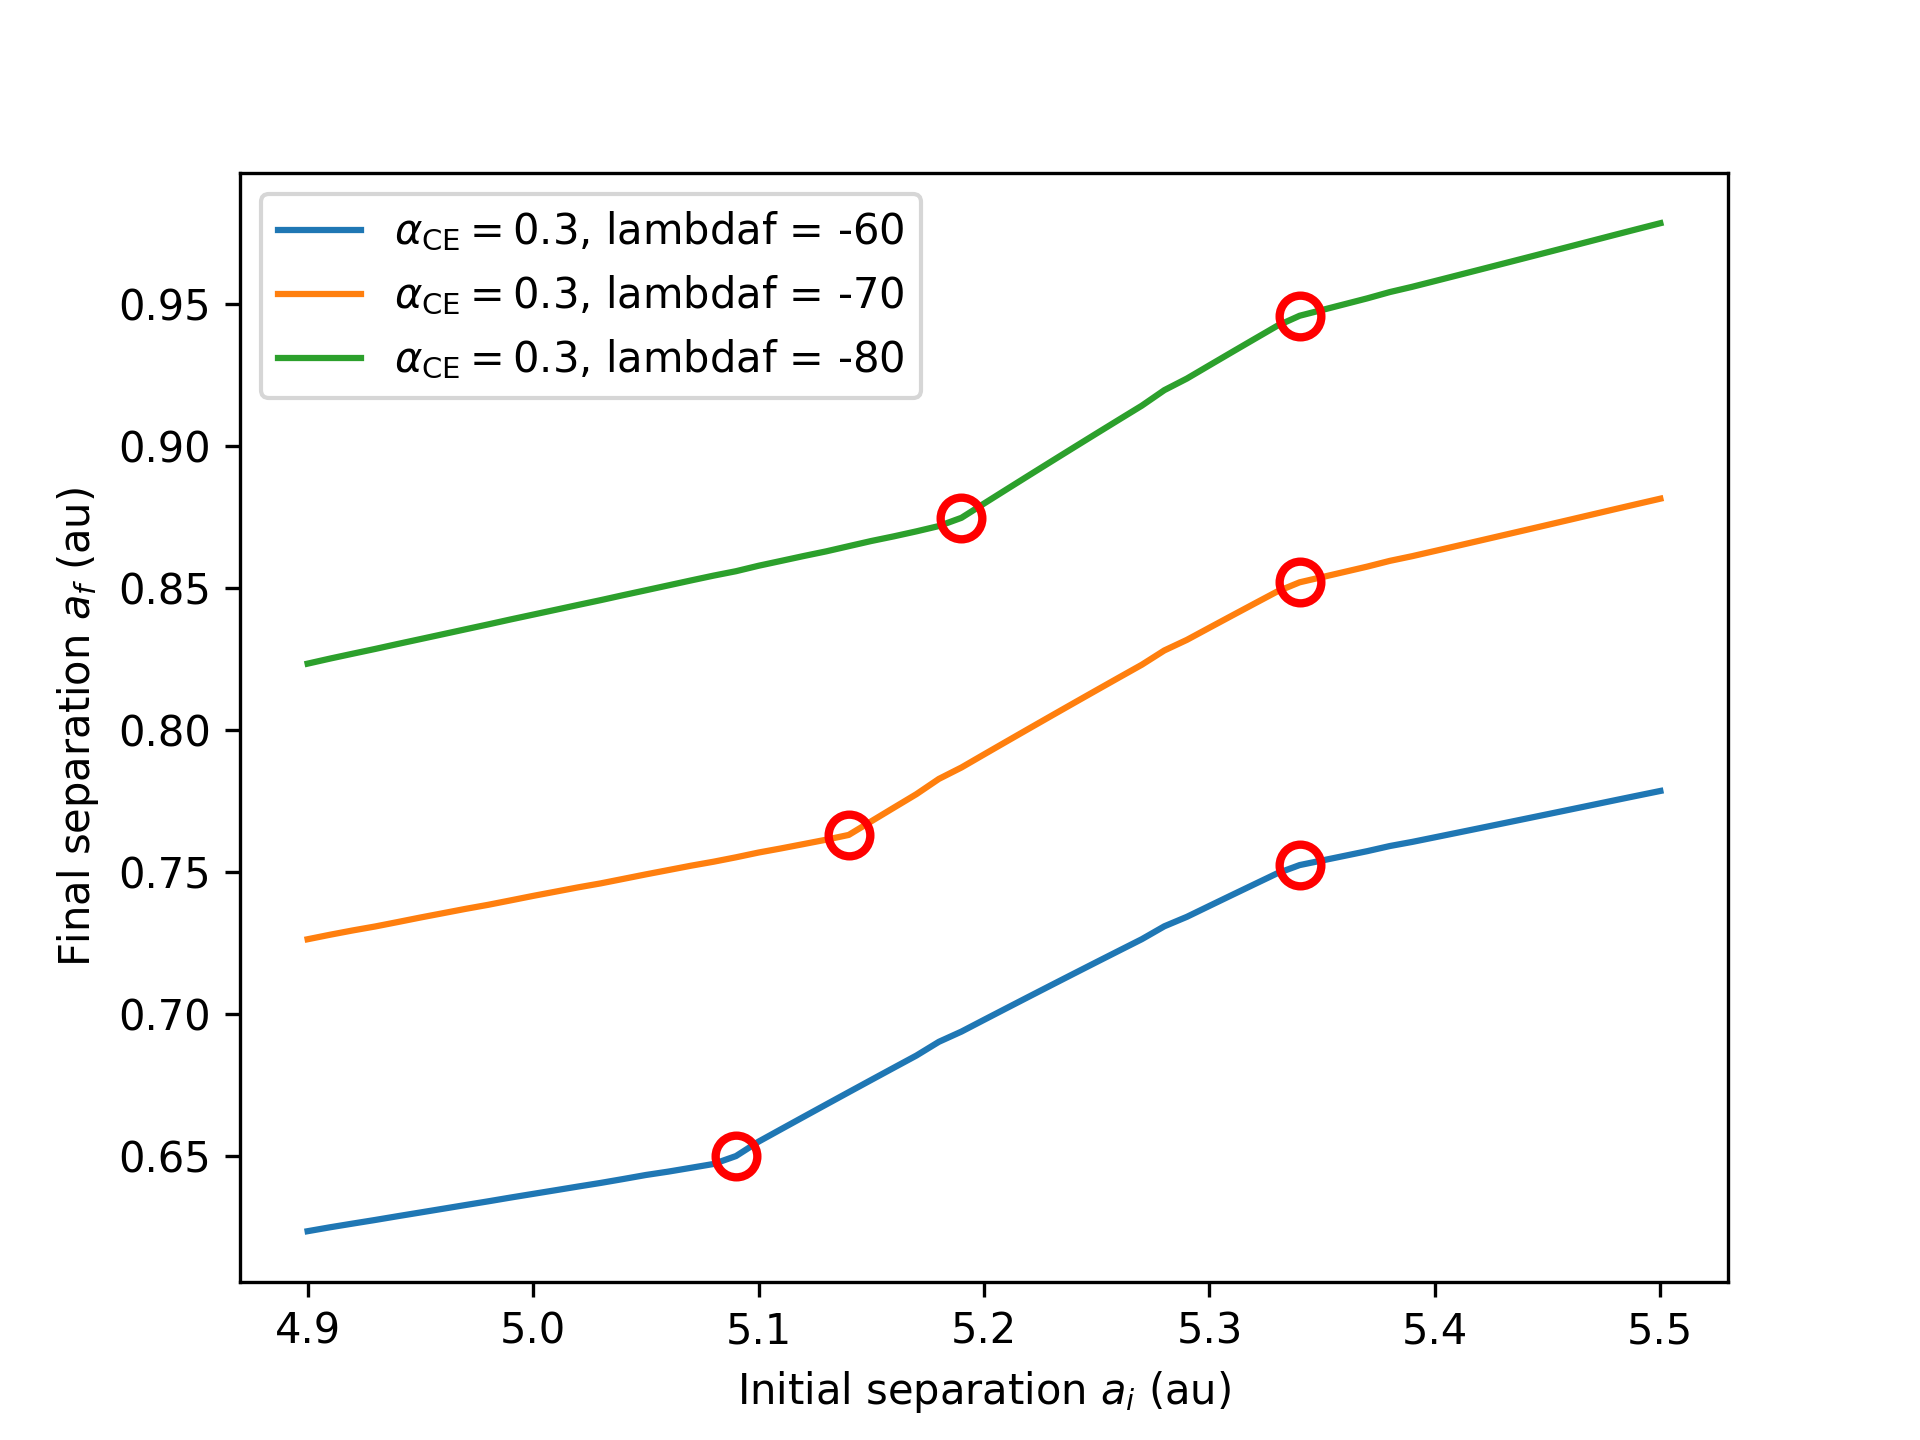
\includegraphics[width = 0.6\linewidth]{jump-zoom.png}
    \caption{Dependence of final separation $a_f$ on initial separation $a_i$ for $\alphace = 0.3$. Simulation results of $\lambda_f = 60$, $70$, and $80$ are shown. The red circles emphasizes the jump of final separation as initial separation increases.}
    \label{jump-zoom}
\end{figure}

Inspecting more closely, we find that the final separation $a_f$ jumps at about $5.2 \sim 5.4 \au$. This is especially obvious with $\alphace = 0.3$. To illustrate, we zoom in the simulation results of $\alphace = 0.3$, and present the change of final separation $a_f$ as initial separation $a_i$ increases in Figure \ref{jump-zoom}. From here, we can clearly see two jumps — one between $5.1\au$ and $5.2\au$, the other at $5.34\au$. To explain this, we again go to the \verb|bpp| array of these systems. We notice that the first jump is probably because the evolution process changes from \textbf{3-7-8-4-3-7-8-4} to \textbf{3-7-8-7-8-4}. This means that for relatively larger initial separation $a_i$, the primary fills its Roche lobe all the time, leading to more mass loss during a shorter timescale and thus larger final separation. Also, the second jump is probably because \verb|kstar_1| changes from \verb|8| (Naked Helium Star Hertzsprung Gap) to \verb|9| (Naked Helium Star Giant Branch) at the start of the second common envelope. This changes the binding energy of the common envelope and thus changes the final separation.

Finally, notice that a small triangular gap in the figure for $\alphace = 1$. This is because \verb|kstar_1| becomes a neutron star and no rows in the \verb|bpp| gets selected.

In conclusion, with a large \verb|lambdaf|, it is possible to create wide post-mass transfer WD+MS systems with final separation $a_f > 0.15 \au$, which is the minimal separation of our observed objects.

\subsubsection{Comparison}
After we have obtained the simulation results for different initial conditions, now we can calculate the effective $\lambda$ that matches with results in \cite{yamaguchi_hi}. We use the following method to build the connection between COSMIC model and MESA model. For each fixed initial separation $a_i$, we loop through the COSMIC results with the same initial separation, and find the \verb|lambdaf| value that results in a final separation closest to MESA model results, documented in the figures of \cite{yamaguchi_hi}. We record this \verb|lambdaf| as the effective $\lambda$ that matches the binding energy formalism at initial separation $a_i$.

For $\Ebind = \Egrav + \Eint$, the fitting results is presented in Figure \ref{fit_hi}, where each line corresponds to different common envelope efficiencies $\alphace$ and different energy budgets (either $\Egrav$ only or $\Egrav + \Eint$).

\begin{figure}
    \centering
    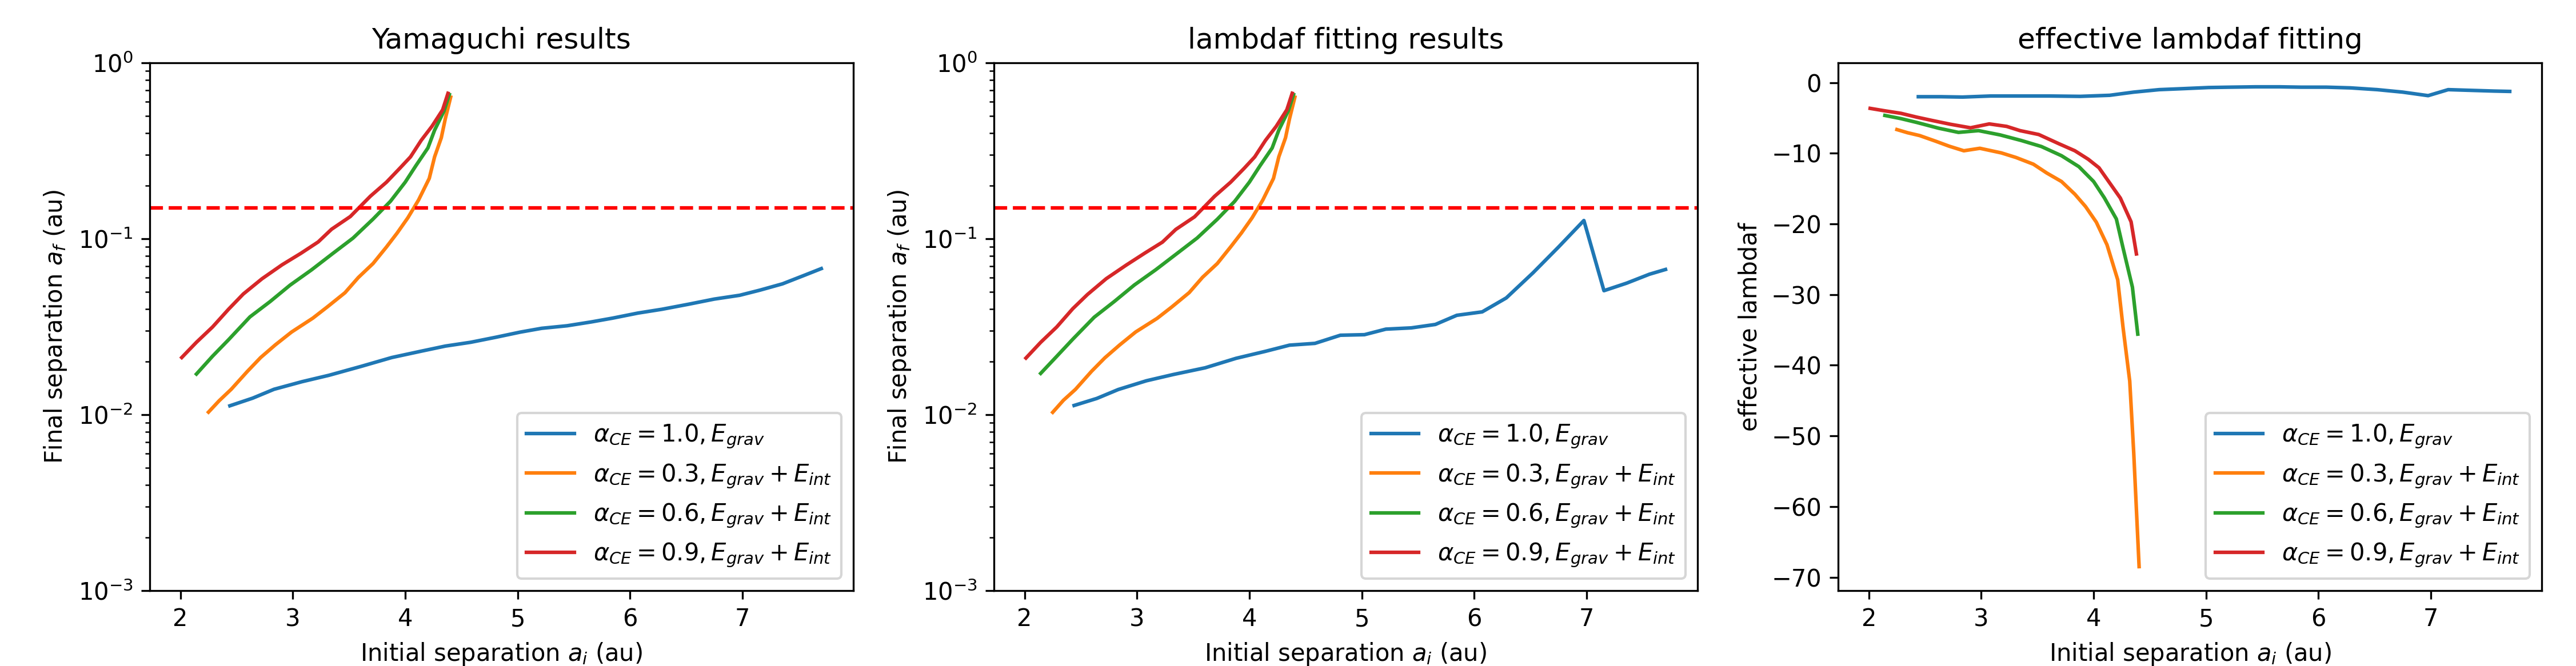
\includegraphics[width=1\linewidth]{7+1fit.png}
    \caption{Effective $\lambda$ fitting results of a $7\Msun + 1\Msun$ system for common envelope structure in MESA. \emph{Left:} MESA results in \cite{yamaguchi_hi} of how final separation $a_f$ depends on initial separation $a_i$. \emph{Center:} COSMIC results of how final separation $a_f$ depends on initial separation $a_i$, produced by the effective $\lambda$. \emph{Right:} effective $\lambda$ in COSMIC that corresponds to the MESA results for each initial separation $a_i$. The red line in the left and middle panel represents $0.15 \au$, the minimal separation for observed wide post-CE WD+MS binaries.}
    \label{fit_hi}
\end{figure}

Notice that there is a small bump in the blue line. This is because at $6 \sim 7 \au$, we cannot reach such low final separation in COSMIC while forming a WD+MS binary at the same time. In the left panel which shows the MESA results documented in \cite{yamaguchi_hi}, we notice that even with low common envelope efficiencies, it is possible to create WD+MS binaries with final separation $>0.15 \au$ in MESA as long as internal energy $\Eint$ is included. However, in the right panel we show that this correspond to very large \verb|lambdaf| in COSMIC ($\lambda > \sim 20$).

To further compare with the default $\lambda$ value in COSMIC, we include in the right panel an extra line which represents the default $\lambda$ value in COSMIC. This default $\lambda$ in the COSMIC model is calculated following Appendix A of \cite{claeys2014theoretical}. For all of our case, we have $M_{\mathrm{env}} > 1$. The results is shown in Figure \ref{fit_cmp_hi}. Notice that the default $\lambda$ value is at order $\sim 1$, far smaller than the effective $\lambda$ needed to recreate results in \cite{yamaguchi_hi}.

\begin{figure}
    \centering
    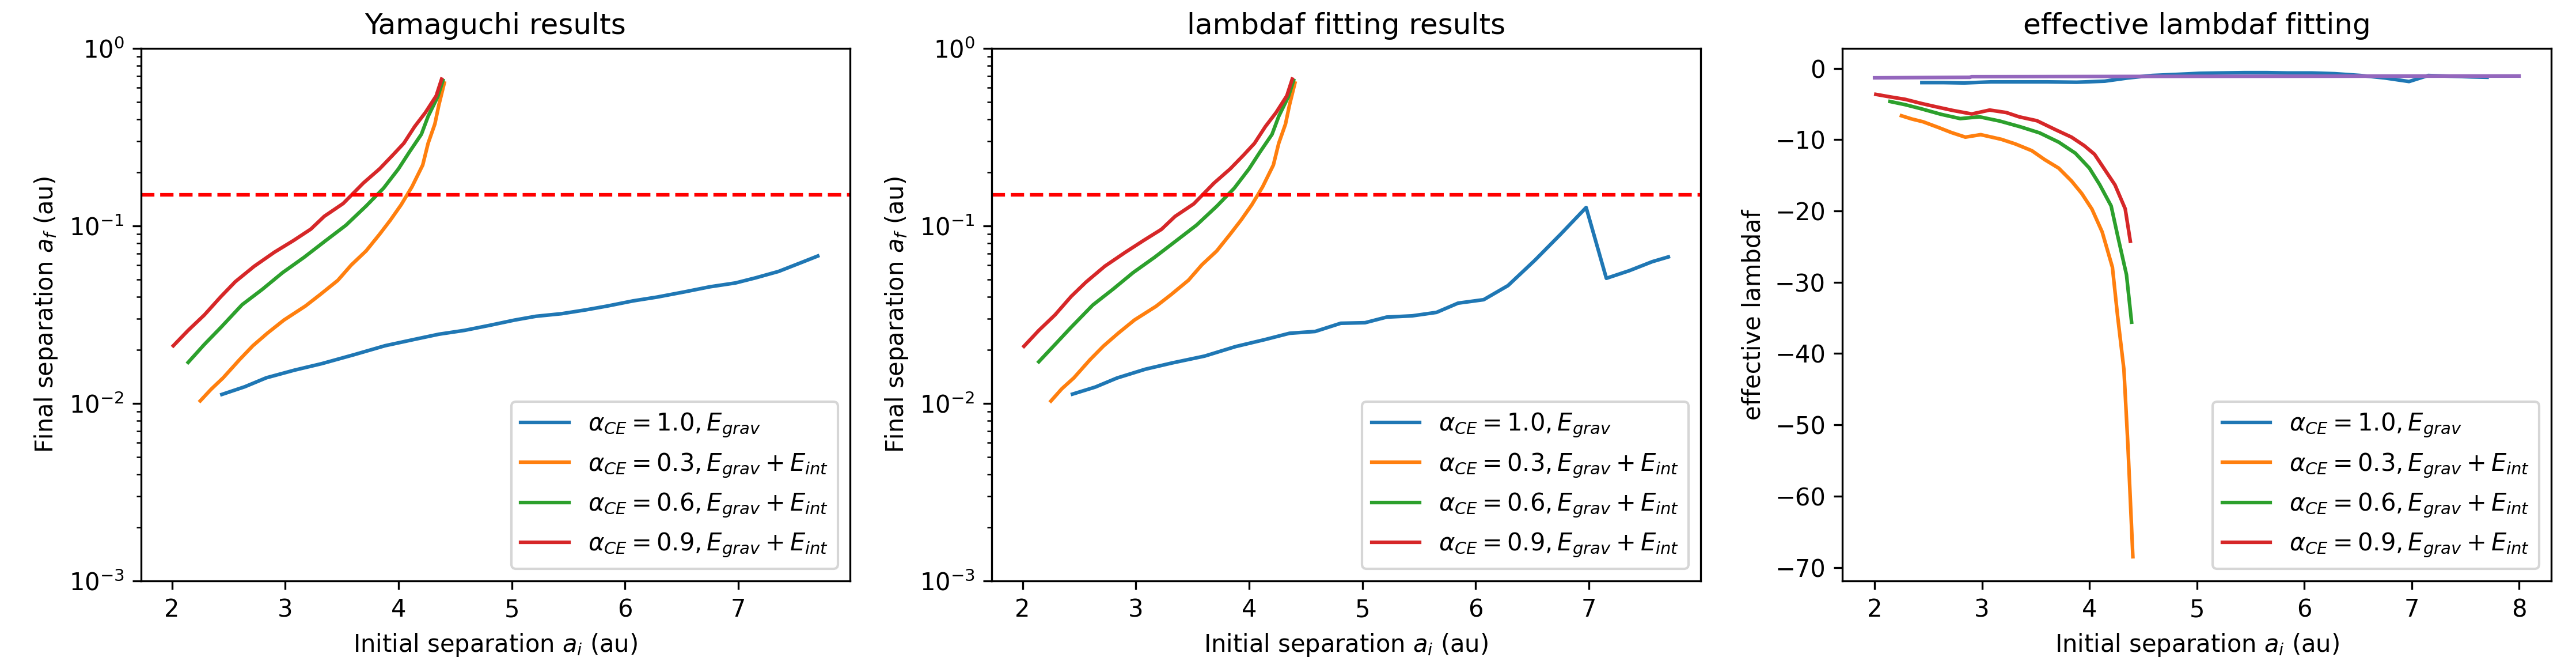
\includegraphics[width=\linewidth]{7+1cmp.png}
    \caption{Same as Figure \ref{fit_hi}, but with default $\lambda$ in COSMIC model included in the right panel.}
    \label{fit_cmp_hi}
\end{figure}

For a different energy budge with $\Ebind = \Egrav + \alphath \Eth + \alpharec \Erec$, the same results is shown in Figure \ref{fit_cmp_eb_hi}

\begin{figure}
    \centering
    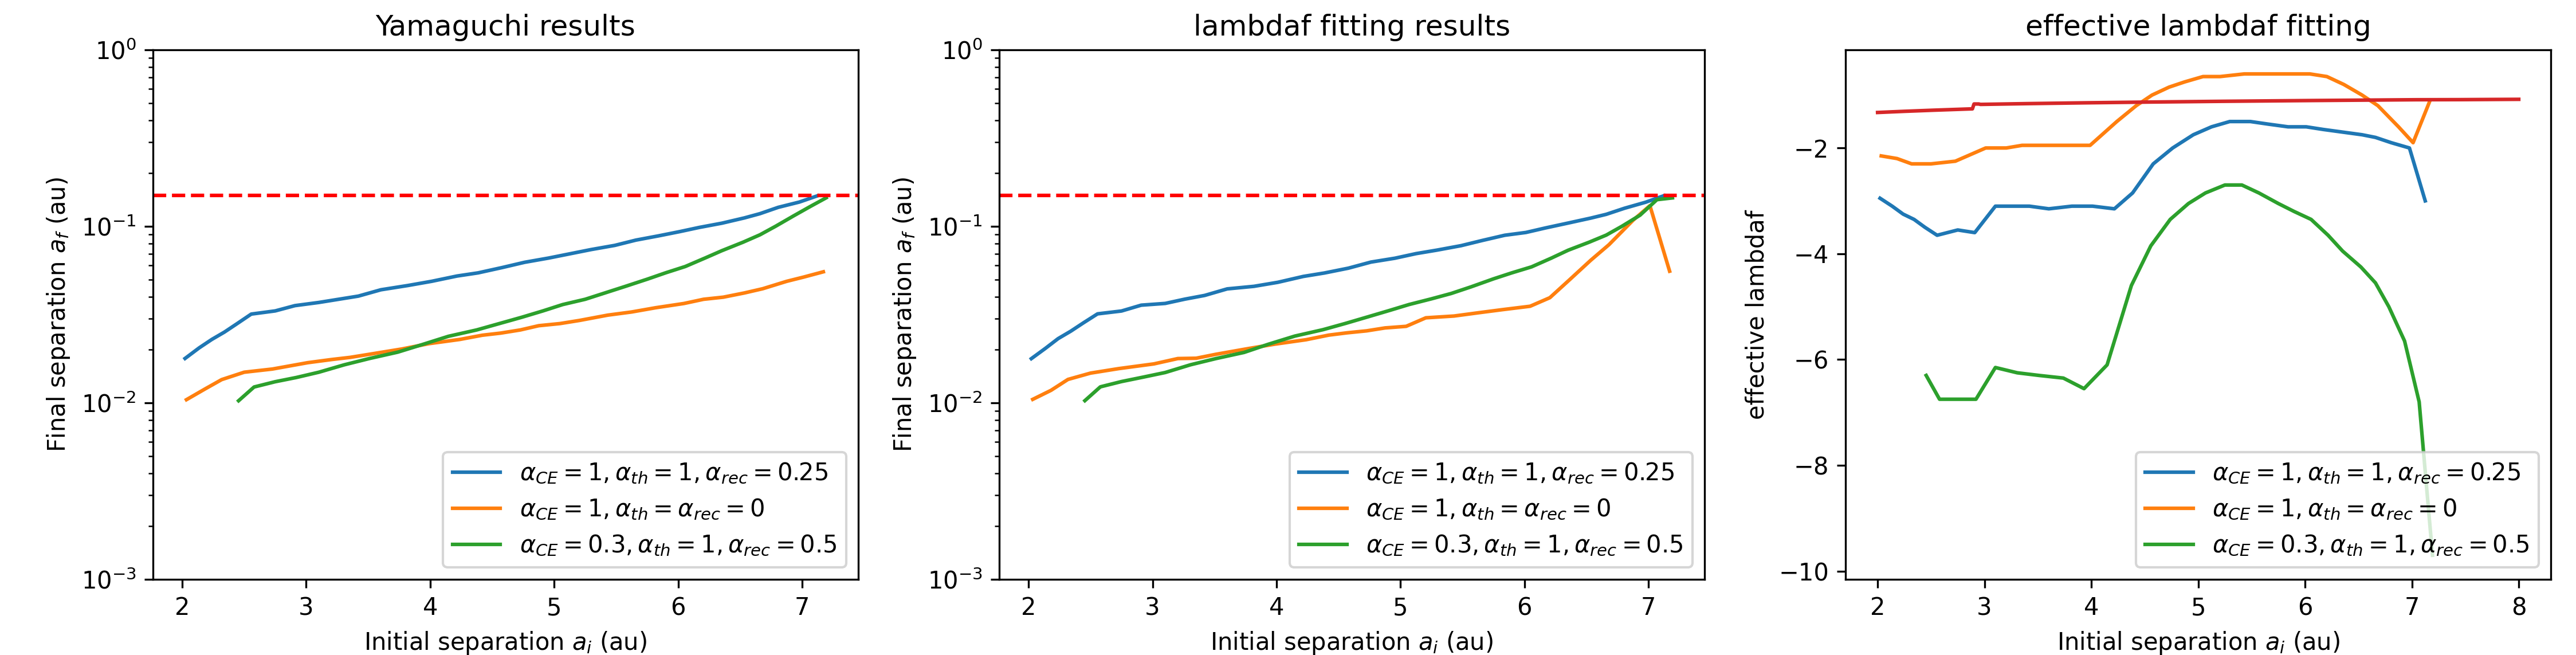
\includegraphics[width=\linewidth]{7+1ebcmp.png}
    \caption{Same as Figure \ref{fit_cmp_hi}, but with a different energy budget.}
    \label{fit_cmp_eb_hi}
\end{figure}


\subsection{Low mass systems ($1.5\Msun + 0.85\Msun$)}

In \cite{yamaguchi_lo}, the author discussed the formation of WD+MS binaries through common envelope for low mass systems ($1.5\Msun + 0.85\Msun$). In this paper, the companion mass is set to be the median of observed systems $\Mstar = 0.85\Msun$, and the progenitor mass fot the WD is expected to be $1 \sim 3 \Msun$. Hence, $1\Msun$, $1.5\Msun$, and $3\Msun$ models are run in MESA. For the energy budget, thermal energy $\Eth$ is fully included while the recombination energy $\Erec$ is included in part with a parameter $\alpharec$. That is,
\[
    \Ebind = \Egrav + \Eth + \alpharec \Erec.
\]
 
The results of MEsA models are shown in Figure \ref{yam_lo}

\begin{figure}
    \centering
    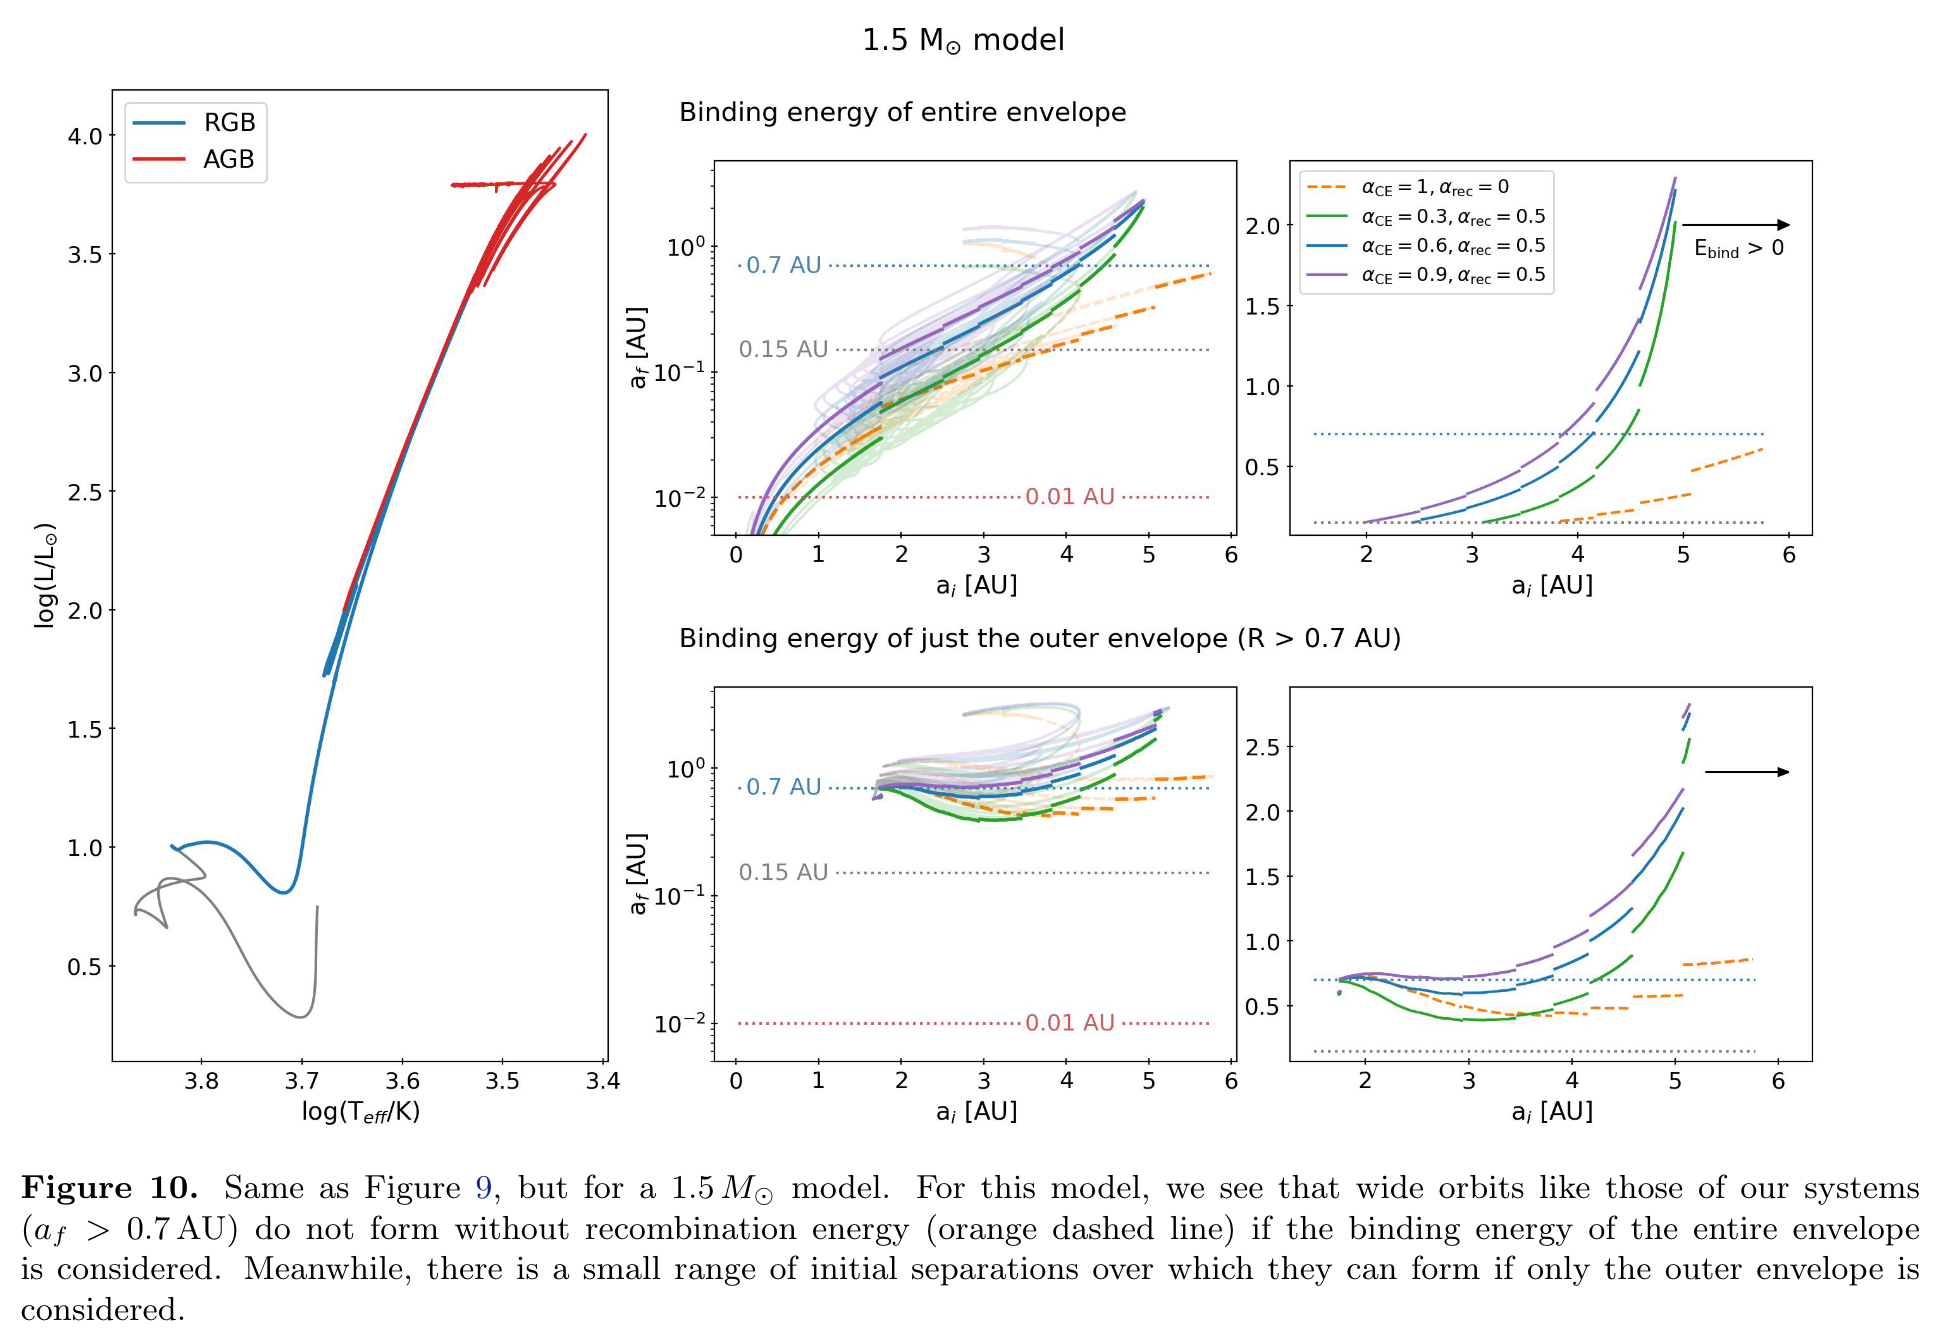
\includegraphics[width=\linewidth]{yamaguchi-1.5+0.8.png}
    \caption{Results of how final separation $a_f$ after common envelope depends on initial separation $a_i$ for different common envelope efficiencies and energy budgets in \cite{yamaguchi_lo}. Here, for final separation $a_f <0.01\au$, WD+MS binaries are not possible, while $0.15\au$ is the observed minimal separation and $0.7\au$ is the typical separation.}
    \label{yam_lo}
\end{figure}

We take the same approach as in high mass systems to investigate the effective structural parameter $\lambda$ that matches with the common evenlope model in MESA. We ran COSMIC binary evolution model for a system of $1.5\Msun + 0.85\Msun$ for different initial separation $a_i$ and \verb|lambdaf|, to investigate how they affect the final separation $a_f$. The results in shown in Figure \ref{res_lo}.

\begin{figure}
    \centering
    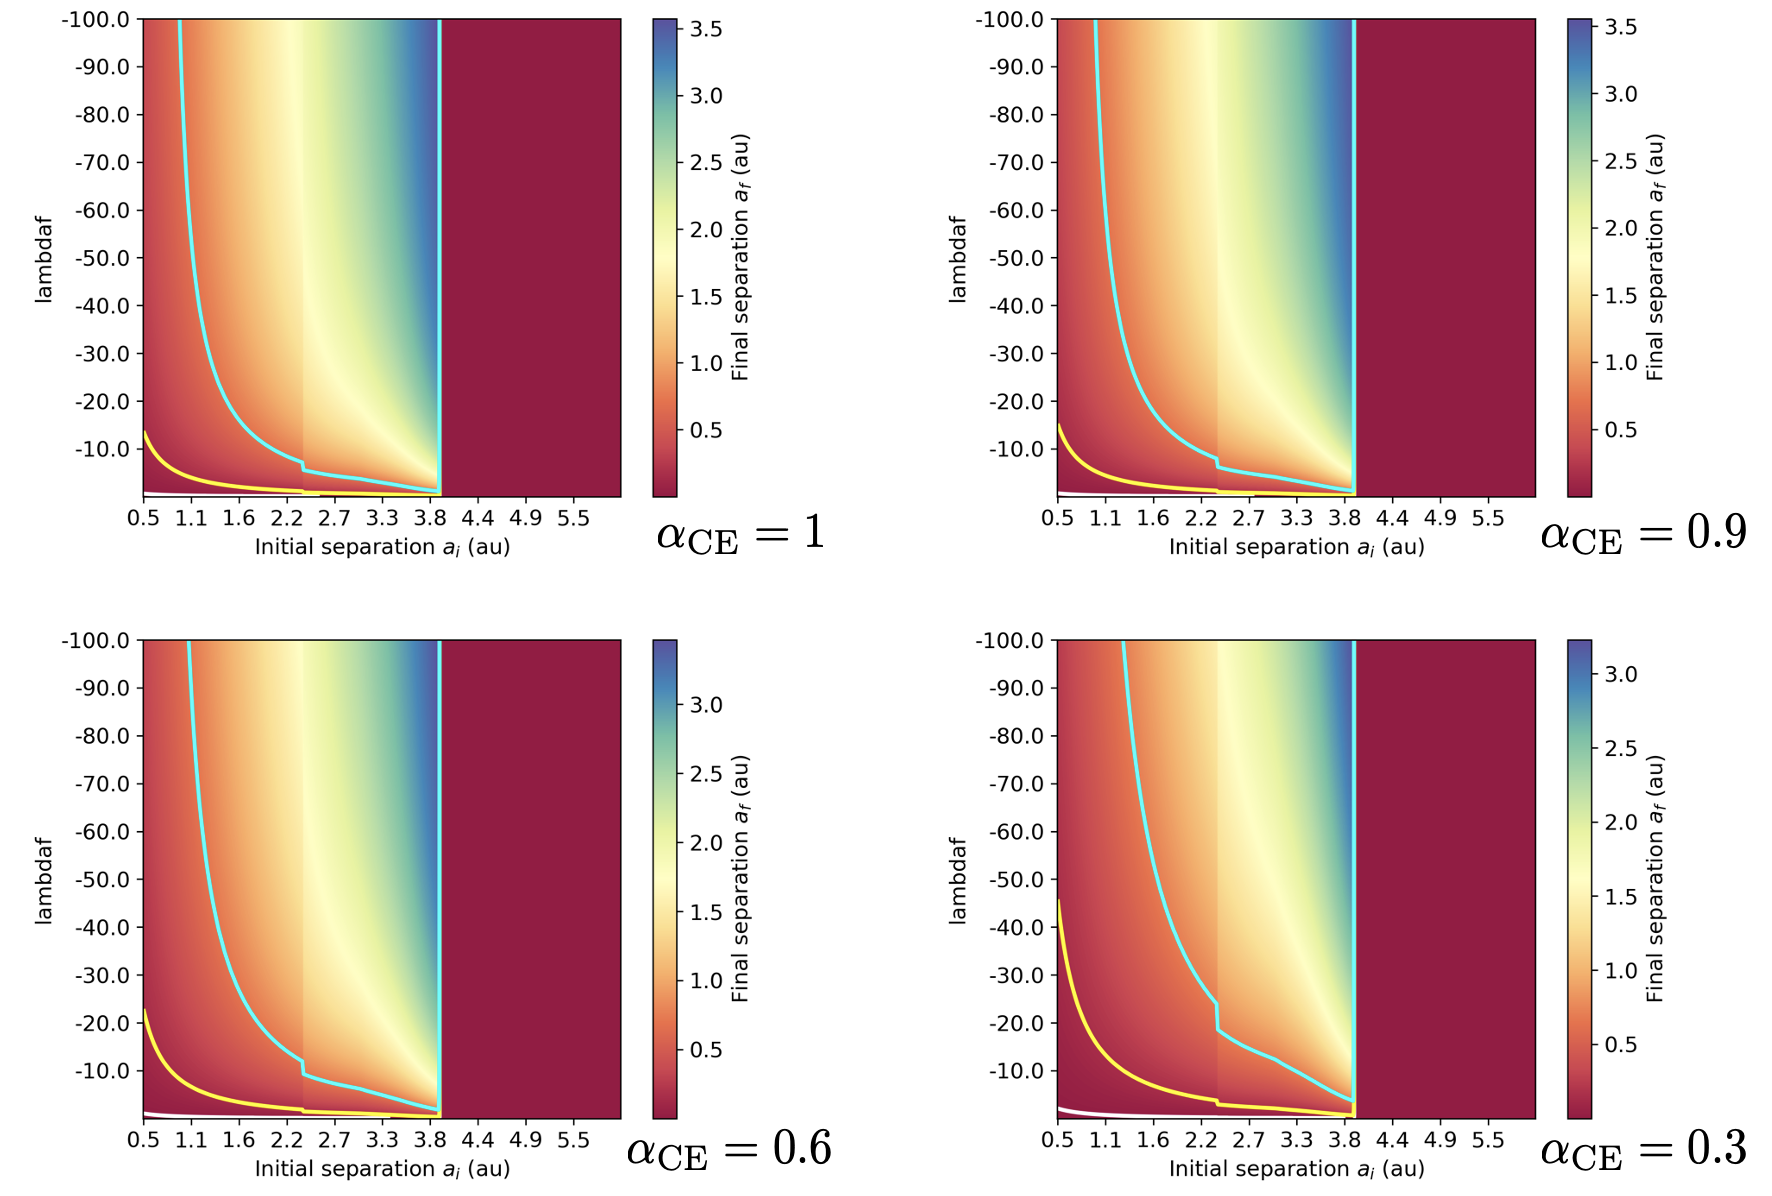
\includegraphics[width=0.9\linewidth]{1.5+0.8results.png}
    \caption{COSMIC results of how final separation $a_f$ depends on initial separation $a_i$ and common envelope flag "lambdaf" for different common envelope efficiencies $\alphace$, where the black and red contour corresponds to $0.01 \au$, $0.15 \au$, and $0.7 \au$ as in Figure \ref{yam_lo} respectively. Outside the black contour no desired system forms since WD+MS binaries are not possible for $a_f < 0.01\au$. $0.15\au$ and $0.7\au$ are the observed minimal separation and the typical separation respectively.}
    \label{res_lo}
\end{figure}

We compare this result with results in \cite{yamaguchi_lo} using the same appraoch as high mass systems. In the paper, the author presents separate results for two different method of calculating the binding energy. One of them contains binding energy of the entire envelope and the other only contains binding energy of the outer envelope. In Figure \ref{fit_cmp_lo_whole}, we compare COSMIC with MESA model that includes binding enregy of the entire envelope. In Figure \ref{fit_cmp_lo_pt}, we compare with with MESA model that includes only binding energy of the outer envelope. Notice that we do not have fitting results for $a_i > 4 \au$. This is because we do not get any WD+MS binaries in COSMIC for such initial separation range.

\begin{figure}
    \centering
    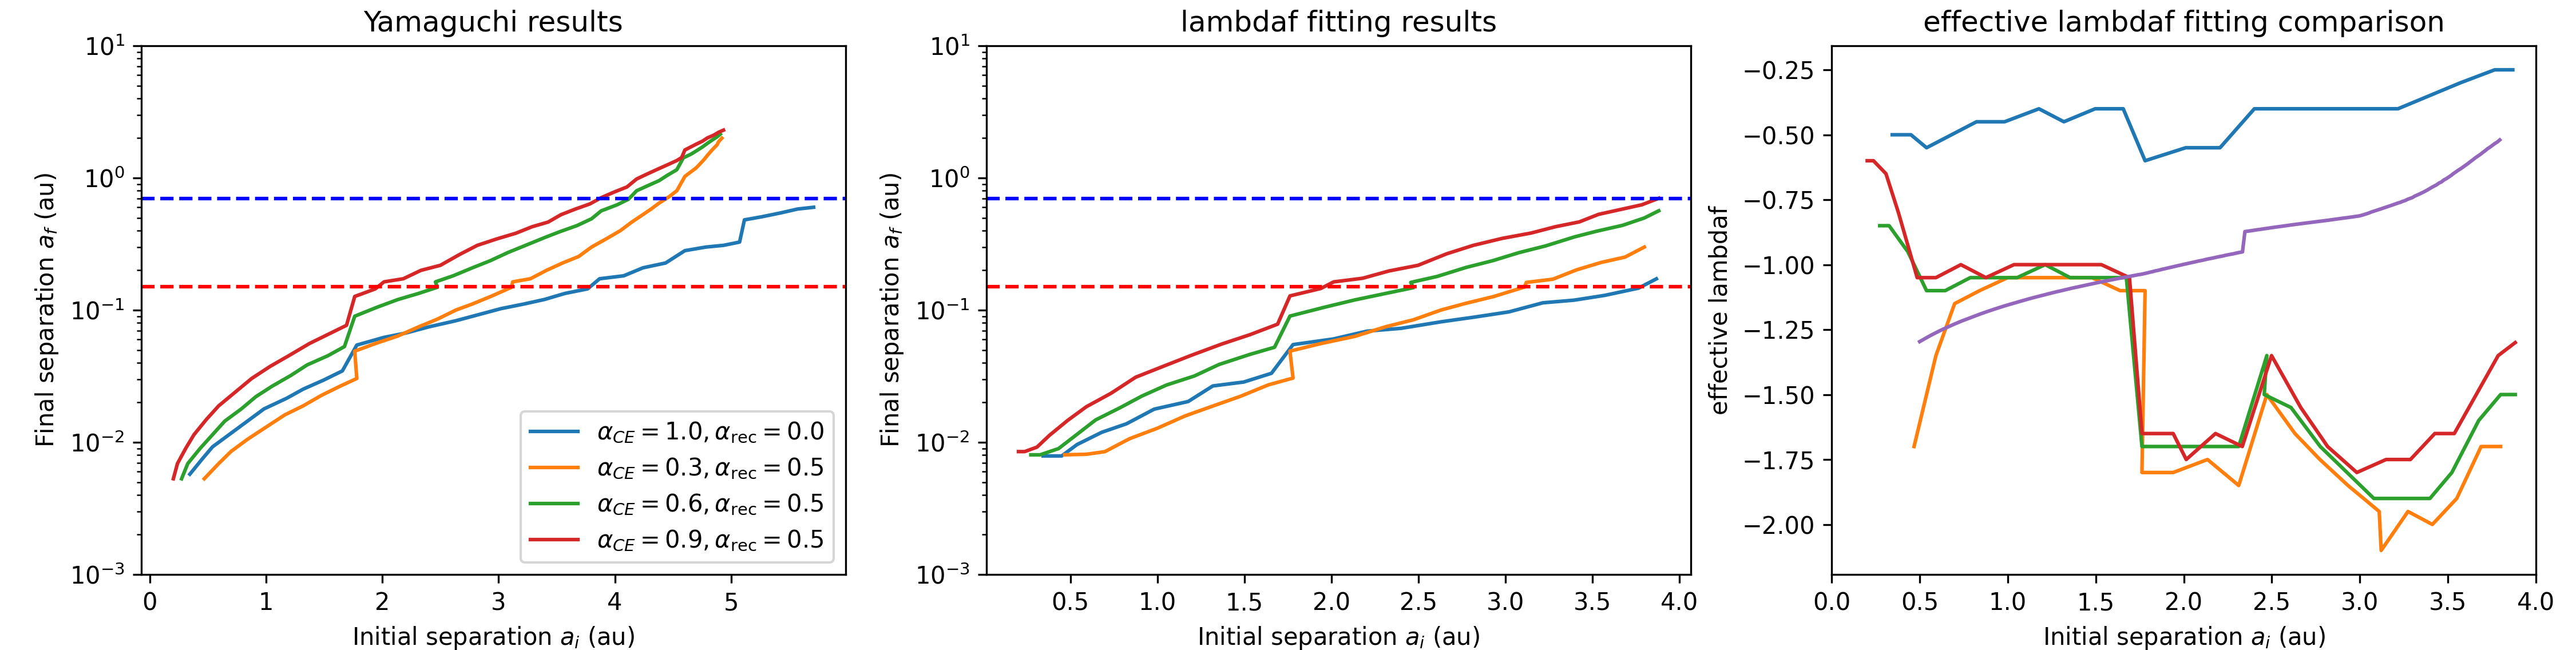
\includegraphics[width=\linewidth]{1.5+0.8cmp_whole.png}
    \caption{Effective $\lambda$ fitting results of a $1.5\Msun + 0.85\Msun$ system for common envelope structure in MESA. Binding energy of the \textbf{entire envelope} is considered. \emph{Left:} MESA results in \cite{yamaguchi_lo} of how final separation $a_f$ depends on initial separation $a_i$. \emph{Center:} COSMIC results of how final separation $a_f$ depends on initial separation $a_i$, produced by the effective $\lambda$. \emph{Right:} effective $\lambda$ in COSMIC that corresponds to the MESA results for each initial separation $a_i$. The purple line represents default $\lambda$ calculated using \cite{claeys2014theoretical}. The red line and the blue line in the left and middle panel represents $0.15 \au$ and $0.7 \au$ respectively. $0.15 \au$ is the minimal separation for observed wide post-CE WD+MS binaries while $0.7 \au$ is the typical separation for such systems.}
    \label{fit_cmp_lo_whole}
\end{figure}

\begin{figure}
    \centering
    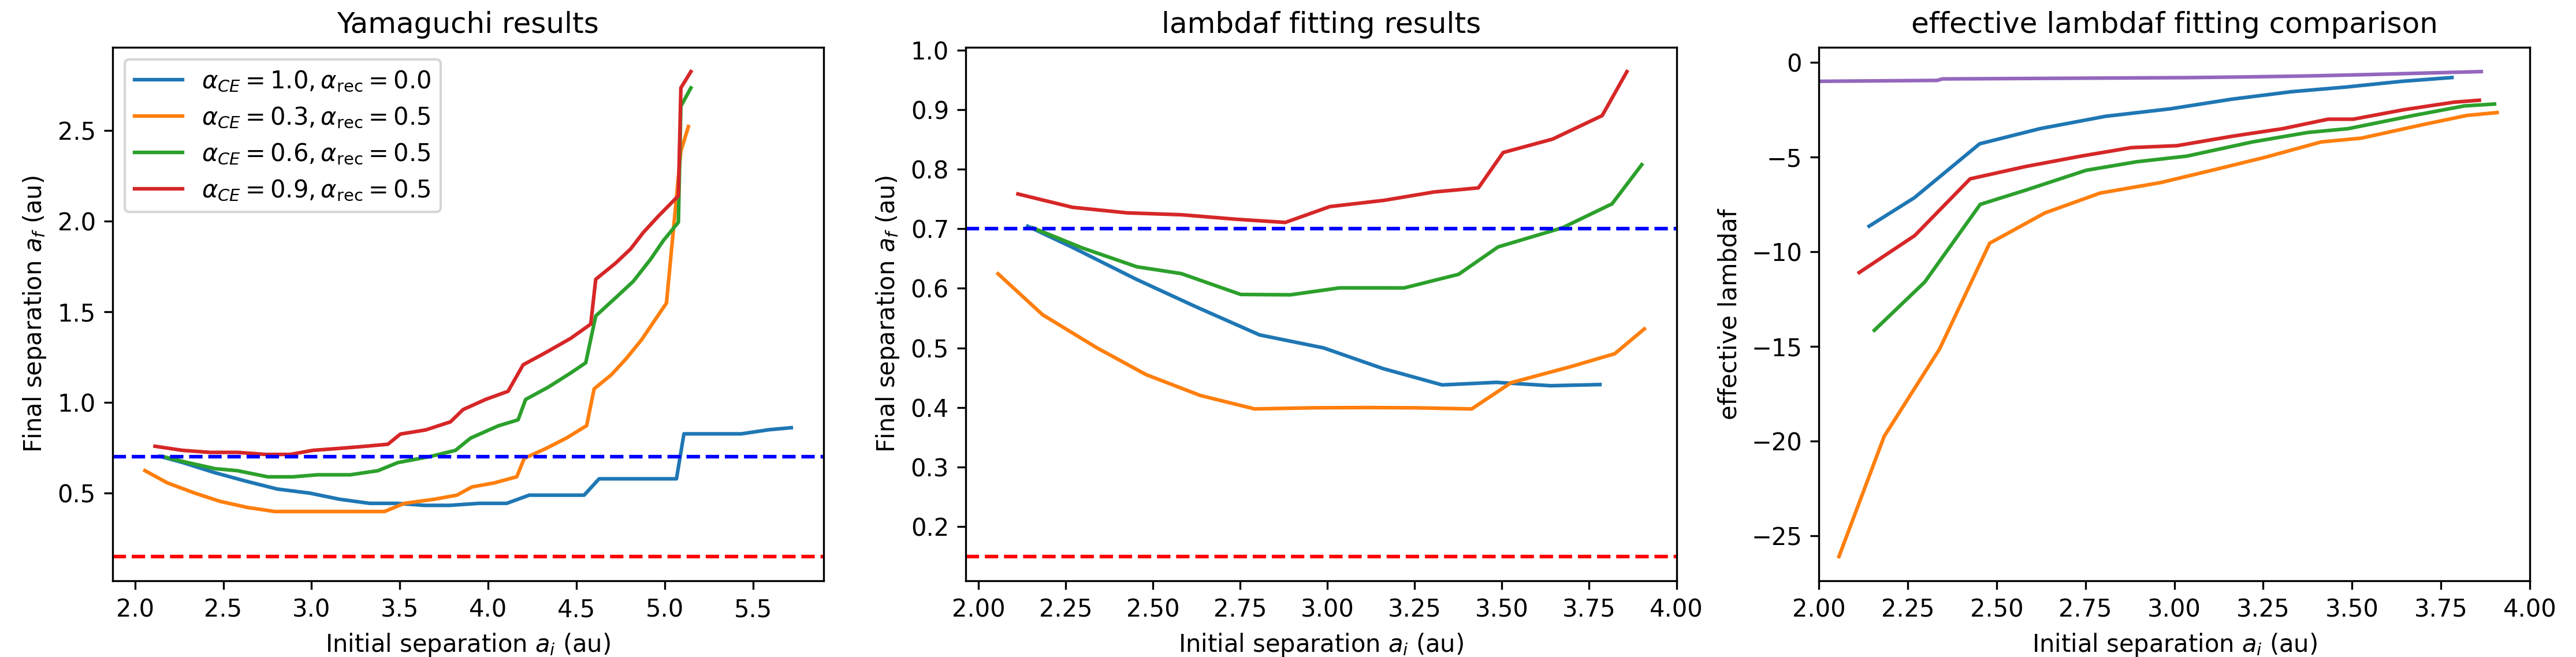
\includegraphics[width=\linewidth]{1.5+0.8cmp_pt.png}
    \caption{Same as Figure \ref{fit_cmp_lo_pt} but only binding enregy of the \textbf{outer envelope} is included.}
    \label{fit_cmp_lo_pt}
\end{figure}

Based on the figure, we find that for low mass systems, the $\lambda$ does not need to be far larger than default to produce WD+MS systems. This is a significant difference between high mass systems and low mass systems.

\section{Stable Mass Transfer}
After exploring the conditions of WD+MS binaries through common envelope, we investigate the possibility of WD+MS binaries formation through stable mass transfer. Similarly, we investigate the condition of forming both high mass systems ($7\Msun + 1\Msun$) and low mass systems ($1.5\Msun + 0.85\Msun$) through stable mass transfer.

\subsection{High mass systems ($7\Msun + 1\Msun$)}

\subsubsection{Methods and results}
First of all, to ensure stable mass transfer, we modify every entry of the \verb|qcrit_array| in \verb|BSEDict| from the default $0.0$ to $20.0$. This will make the actual mass ratio of our system below this critical value for common envelope thorughout the entire process of mass transfer.

Secondly, to investigate dependence on different accretion efficiency, we modify the \verb|acc_lim| flag in \verb|BSEDict|, that is, the fraction $\beta$ of all transfered materials is accreted by the accretor, or $\dot{M_a} = - \beta\dot{M_d}$. For each accretion efficiency, we run COSMIC binary simulation of a $7\Msun + 1 \Msun$ system for initial separation ranging from $2 \au$ to $8 \au$. After the simulatio is finished, we select the first row, if any, that shows a WD+MS binary from \verb|bpp| for each initial separation, and document the final separation. In this way, we can see how final separation depends on the initial separtion, and we can compare them with the observed minimum separation $0.15\au$. 

The results is presented in Figure \ref{stable_hi}. The gap in the center means no WD+MS system forms for that initial separation. In fact, a closer inspection of the \verb|bpp| shows that for these systems, two stars merges. The details of the \verb|bpp| will be discussed in a more detailed manner in the next section.

\begin{figure}
    \centering
    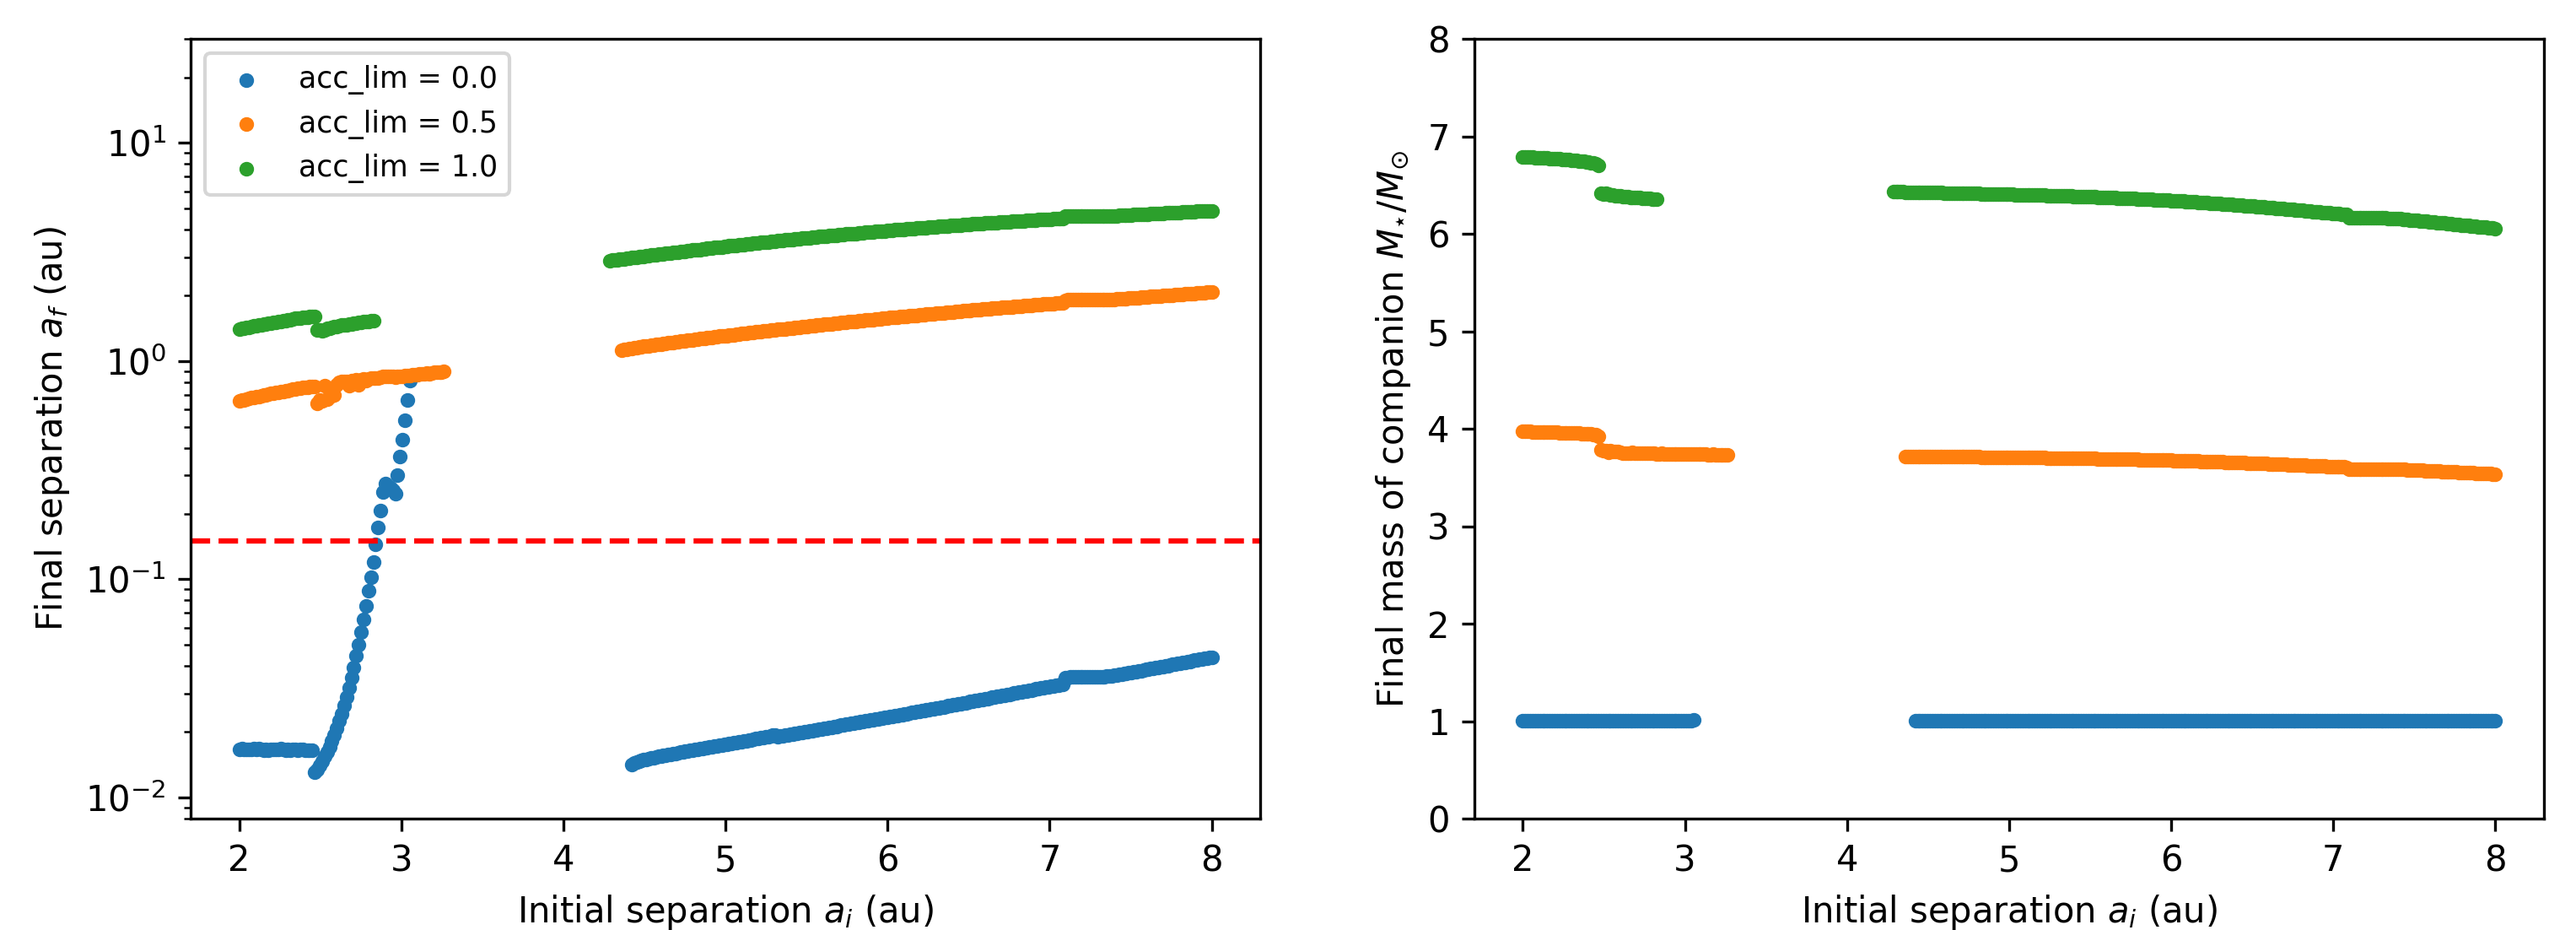
\includegraphics[width=0.75\linewidth]{stable_hi_log.png}
    \caption{COSMIC results of WD+MS binaries after stable mass transfer for $7\Msun + 1\Msun$ systems, with accretion efficiency $\beta = 0$, $\beta = 0.5$, and $\beta = 1$ respectively. \emph{Left:} dependence of final separation $a_f$ of the WD+MS binary on initial separation $a_i$. \emph{Right:} The corresponding companion mass in solar units in the WD+MS binary. The gap in both figure represents that no WD+MS system forms for that initial separation.}
    \label{stable_hi}
\end{figure}

Notice that the majority of these systems have final separation $a_f > 0.15 \au$. However, this is \textbf{not the correct approach}, since the companion mass in our observed wide WD+MS binaries has median mass $\sim 1\Msun$. However, in the simulation results shown in Figure \ref{stable_hi}, the final companion mass is about $4 \Msun$ and $6.5\Msun$ for \verb|acc_lim = 0.5| and \verb|acc_lim = 1.0| respectively. Hence, we need to adjust the  initial companion mass $M_{\star, i}$ and the accretion efficiency \verb|acc_lim|, in order to make the final companion mass $M_{\star, f}$ close to $1\Msun$.

\begin{figure}
    \centering
    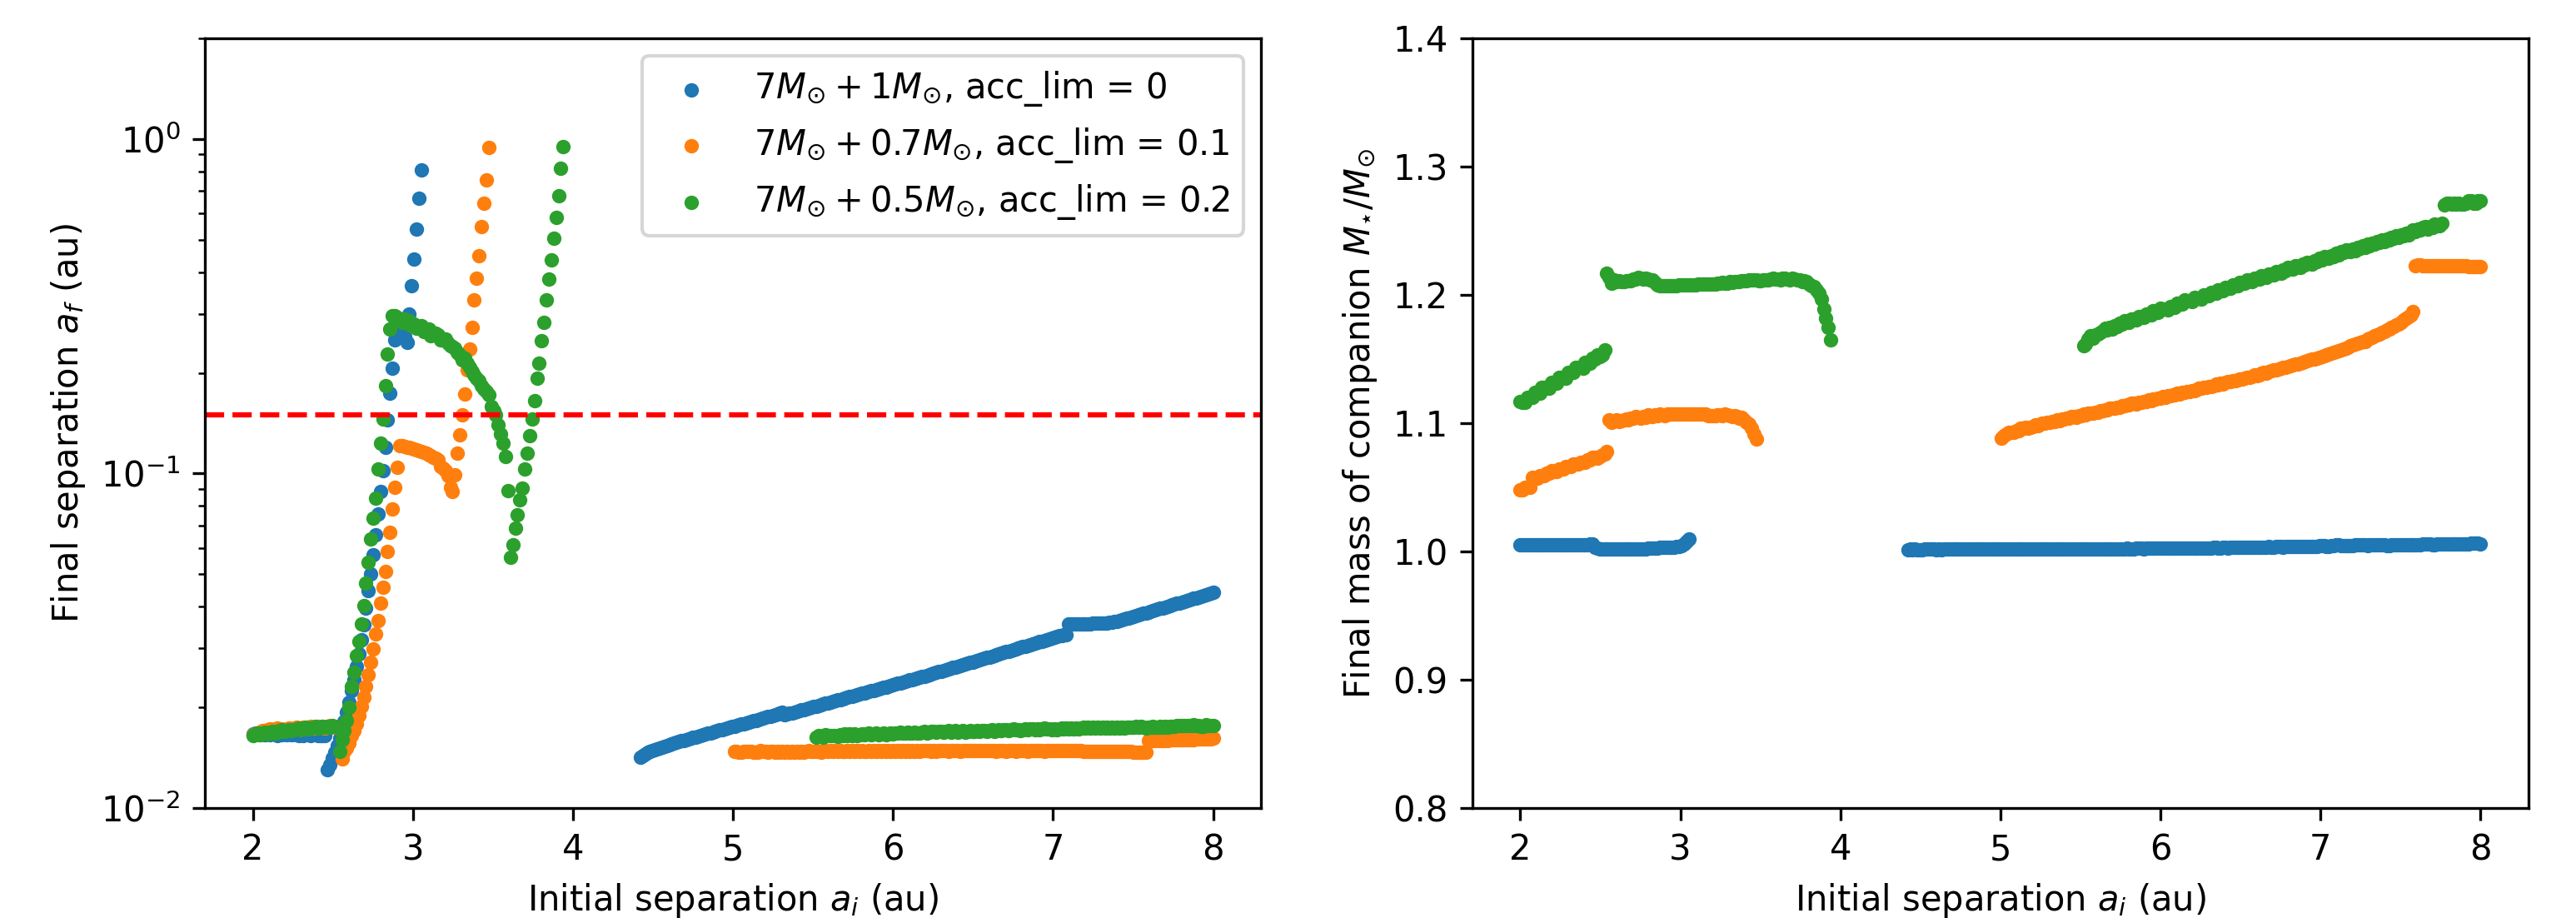
\includegraphics[width = 0.75\linewidth]{stable7+1ex.png}
    \caption{COSMIC results of WD+MS binaries after stable mass transfer for two systems — $7\Msun + 0.7\Msun$ with accretion efficiency $\beta = 0.1$, and $7\Msun + 0.5\Msun$ with accretion efficiency $\beta = 0.2$. The left and right panel presents the same content as in Figure \ref{stable_hi}.}
    \label{stable_hi_ex}
\end{figure}

Therefore, we lower the initial companion mass $M_{\star, i}$ and adjust the accretion efficiency \verb|acc_lim| and re-run the simulation. The results for $7\Msun + 0.7\Msun$ with \verb|acc_lim=0.1|, and $7\Msun + 0.5\Msun$ with \verb|acc_lim = 0.2| is shown in Figure \ref{stable_hi_ex}.

After adjusting the initial mass of companion and the accretion efficiency, now the final mass of the companion is about $1\Msun$ and we get systems similar to our observed sample. Notice that when initial separation $a_i$ is in the range of about $2.5 \au$ to $4.5 \au$, the final separation increases rapidly. Also, it is only in this region that the final separation goes larger than the observed minimum $0.15 \au$. Hence, in the next subsection, we focus on this sharp increase and try to explain it qualitatively.

\subsubsection{Discussions}
In the previous section, we mentioned how $7\Msun + 1 \Msun$ systems with \verb|acc_lim = 0|, $7 \Msun + 0.7\Msun$ systems with \verb|acc_lim = 0.1|, and $7 \Msun + 0.5 \Msun$ systems with \verb|acc_lim = 0.2| produces WD+MS binaries with final separation $a_f > 0.15 \au$ and companion mass $\sim 1 \Msun$ in certain range of initial separation $a_i$. From the figure, we can clearly see that when initial separation $a_i$ is in the range of $2.5 \au \sim 4.5\au$, the final separation increases sharply as initial separation increases. In this section, we investigate the reason behind this by focusing on $7\Msun + 1\Msun$ binaries with \verb|acc_lim = 0|.

First of all, let's take a look at how the final separation $a_f$ depends on the initial separation $a_i$ throughout the range of $2 \sim 8 \au$. In general, as shown in Figure \ref{stable_hi_ex}, the dependence of $a_f$ on $a_i$ can be roughly divided into four parts — \textbf{pre-spike, spike, merge, and after-merge}, which corresponds to the part before the sharp increase ($a_i < 2.5 \au$), the part where final separation increases sharply ($2.5 \au < a_i < 3.5 \au$), the part where the binary merges and no desired system is formed ($3.5 \au < a_i < 4.5 \au$), and the part after that ($a_i > 4.5 \au$).

A typical \textbf{pre-spike} \verb|bpp| is presented in the left panel of Figure \ref{pre-spike-spike}. Notice that the binary come into contact (\verb|evol_type = 5|), which follows by a common envelope phase. The same is observed in \textbf{spike} binaries, as shown in the right panel of \ref{pre-spike-spike}.

\begin{figure}
    \centering
    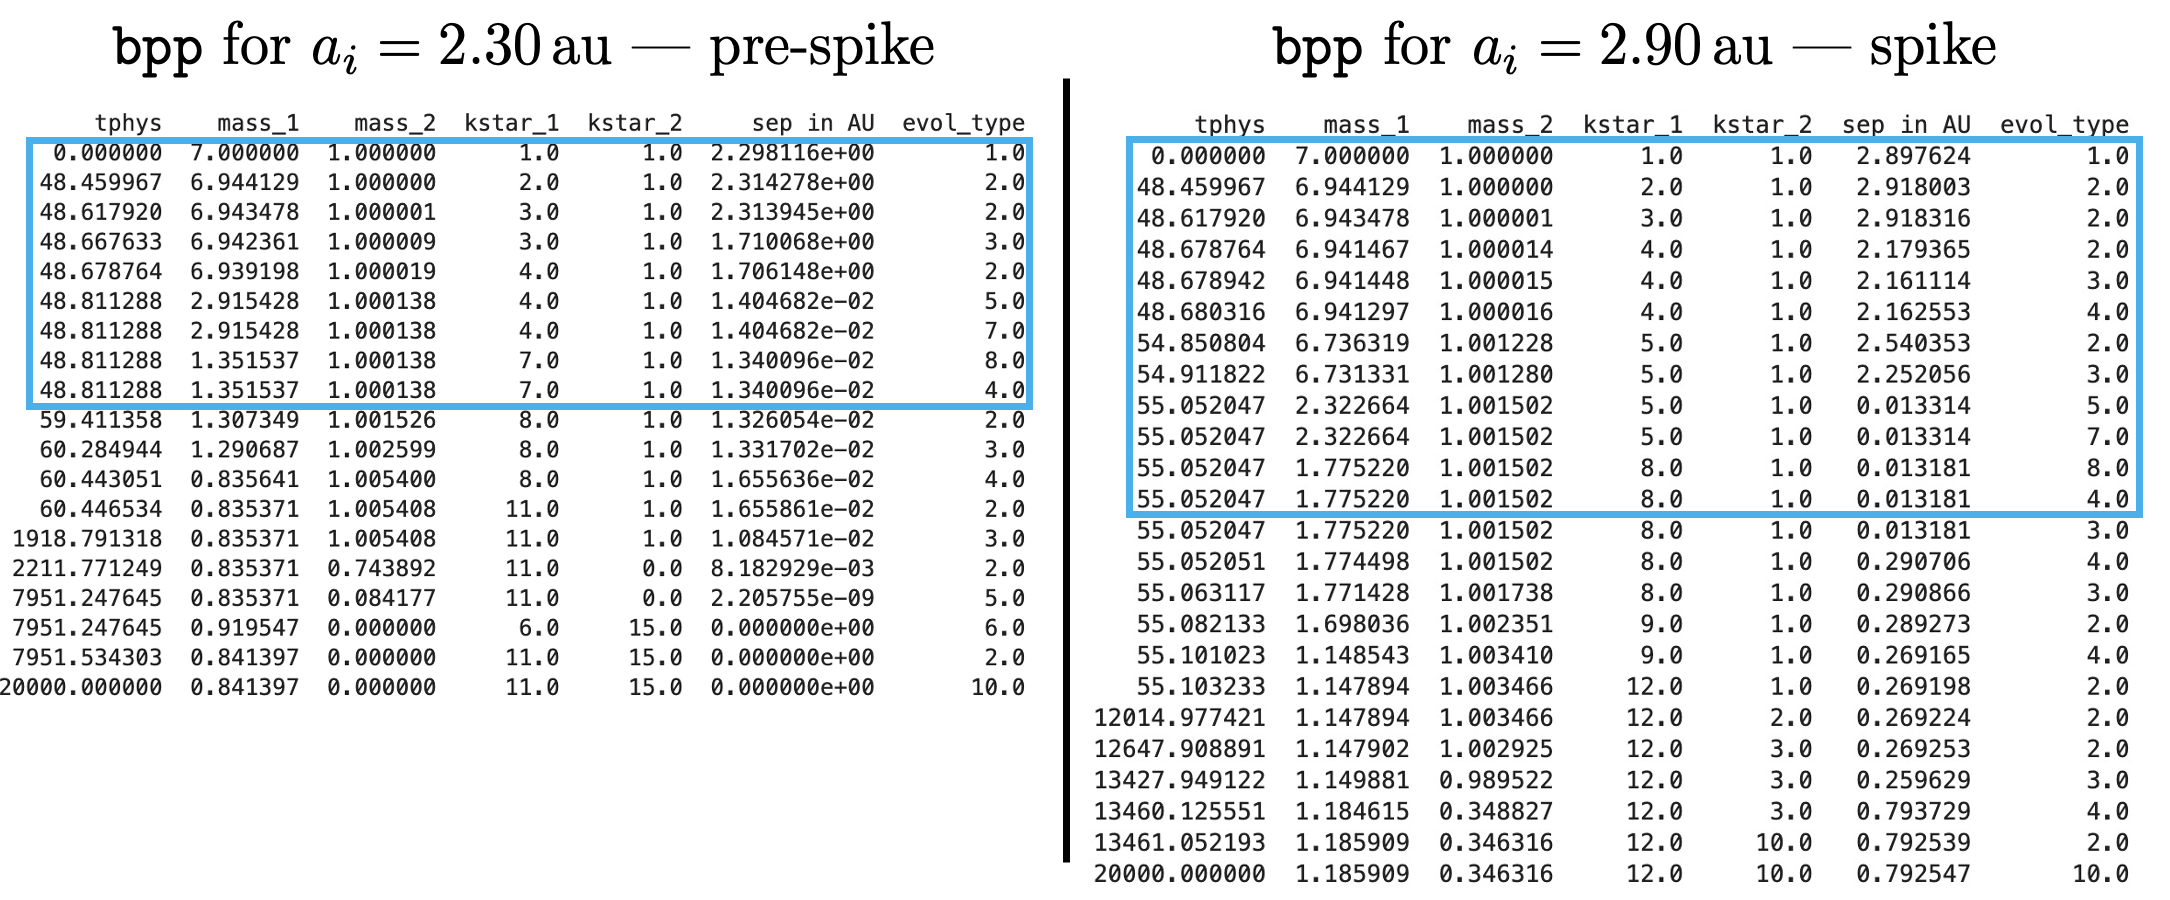
\includegraphics[width=\linewidth]{pre-spike-spike.png}
    \caption{COSMIC simulation data of $7 \Msun + 1 \Msun$ systems with accretion efficiency $\beta = 0$ and initial separation $2.30 \au$ and $2.90 \au$ respectively. They represent typical "pre-spike" binaries and "spike" binaries. The blue rectangle marks out the common first phase of evolution in both systems — contact and common envelope mass transfer.}
    \label{pre-spike-spike}
\end{figure}

Two typical \textbf{spike} \verb|bpp| is presented in Figure \ref{spike}. In the left panel, we notice that the stable mass transfer process in the green rectangle widens the orbit a lot. In the right panel, the extra stable mass transfer process in the red rectangle also significantly widens the orbit. However, in the right panel, the orbit widens without the primary's losing a lot of mass, and the corresponding mass transfer in green does not widen the orbit, even shrinking it.

\begin{figure}
    \centering
    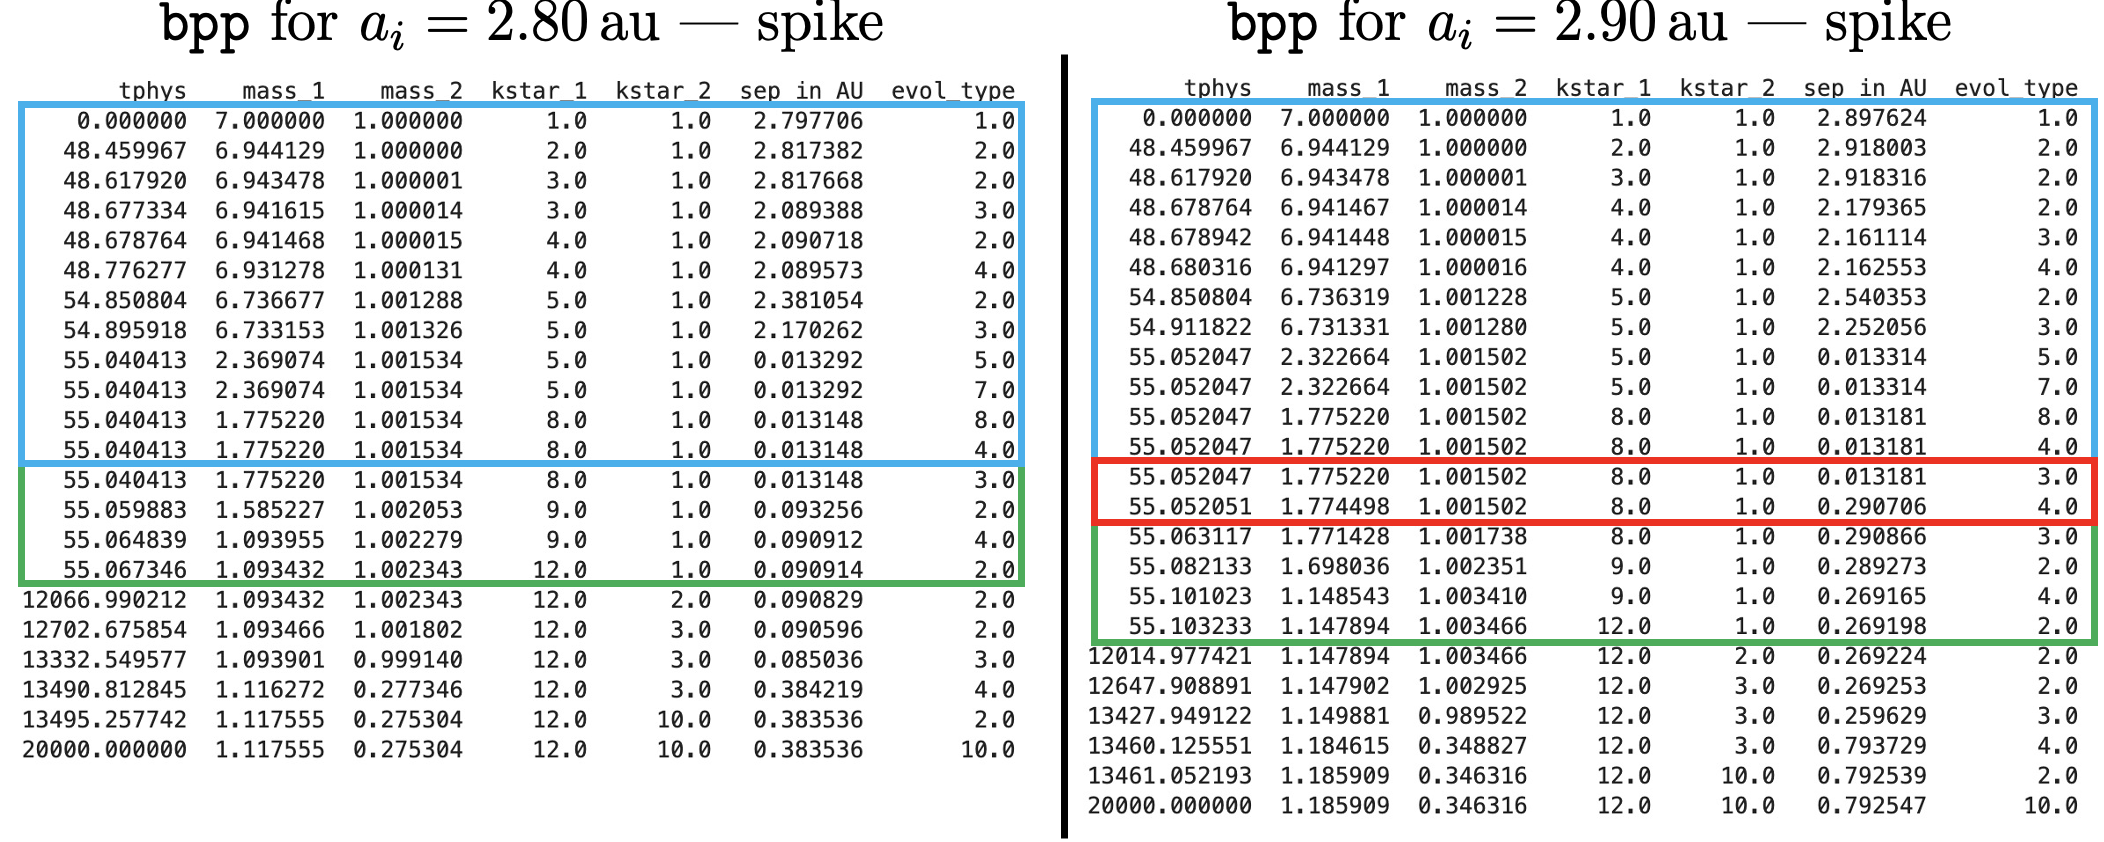
\includegraphics[width=\linewidth]{sharp-inc-bpp.png}
    \caption{COSMIC simulation of systems $7 \Msun + 1 \Msun$ with accretion efficiency $\beta = 0$ and initial separation $2.80 \au$ and $2.90 \au$ respectively. The red rectangle emphasizes the extra mass transfer process that significantly widens the orbit without the primary losing significant mass.}
    \label{spike}
\end{figure}

To qualitatively explain thses results, note first that for a stable and non-conservative and the mass, we have
\[
\frac{\dot J}{J} \propto (1-\beta) q_d \frac{\dot{M_d}}{M_T}.
\]
While $a \sim J^2$, the non-conservative mass transfer should causes the orbit to expand. Note also that mass transfer begins when the primary is a Naked Helium Star on the Hertzsprung Gap (\verb|evol_type = 8|), whose wind mass loss is significant. Also, for wind mass loss, we have
\[
\frac{\dot a}{a} = - \frac{\dot M}{M_T}.
\] 
Therefore, strong wind stripping mass from the primary will cause the orbit to expand even further. To illustrate this more clearly, we change the \verb|windflag| in \verb|BSEDict| to 0, which correspond to weak wind. Now the $a_i = 2.80 \au$ system has final separation $a_f = 0.05 \au$, and the $a_i = 2.90 \au$ system has final separation $a_f = 0.14 \au$, both smaller than the original $0.09 \au$ and $0.27\au$ that correspond to stronger wind.

From the equations, it is not difficult to see that the increase of separation is more obvious for larger separation $a$ for both wind mass loss and stable, non-conservative mass transfer. Therefore, we conclude qualitatively that for \textbf{pre-spike} and \textbf{spike} systems, non-conservative mass transfer and wind mass loss widens the orbit. While this is more obvious for large separation $a$, this accounts for the spike of final separation $a_f$ as the initial separation $a$ increases.

\begin{figure}
    \centering
    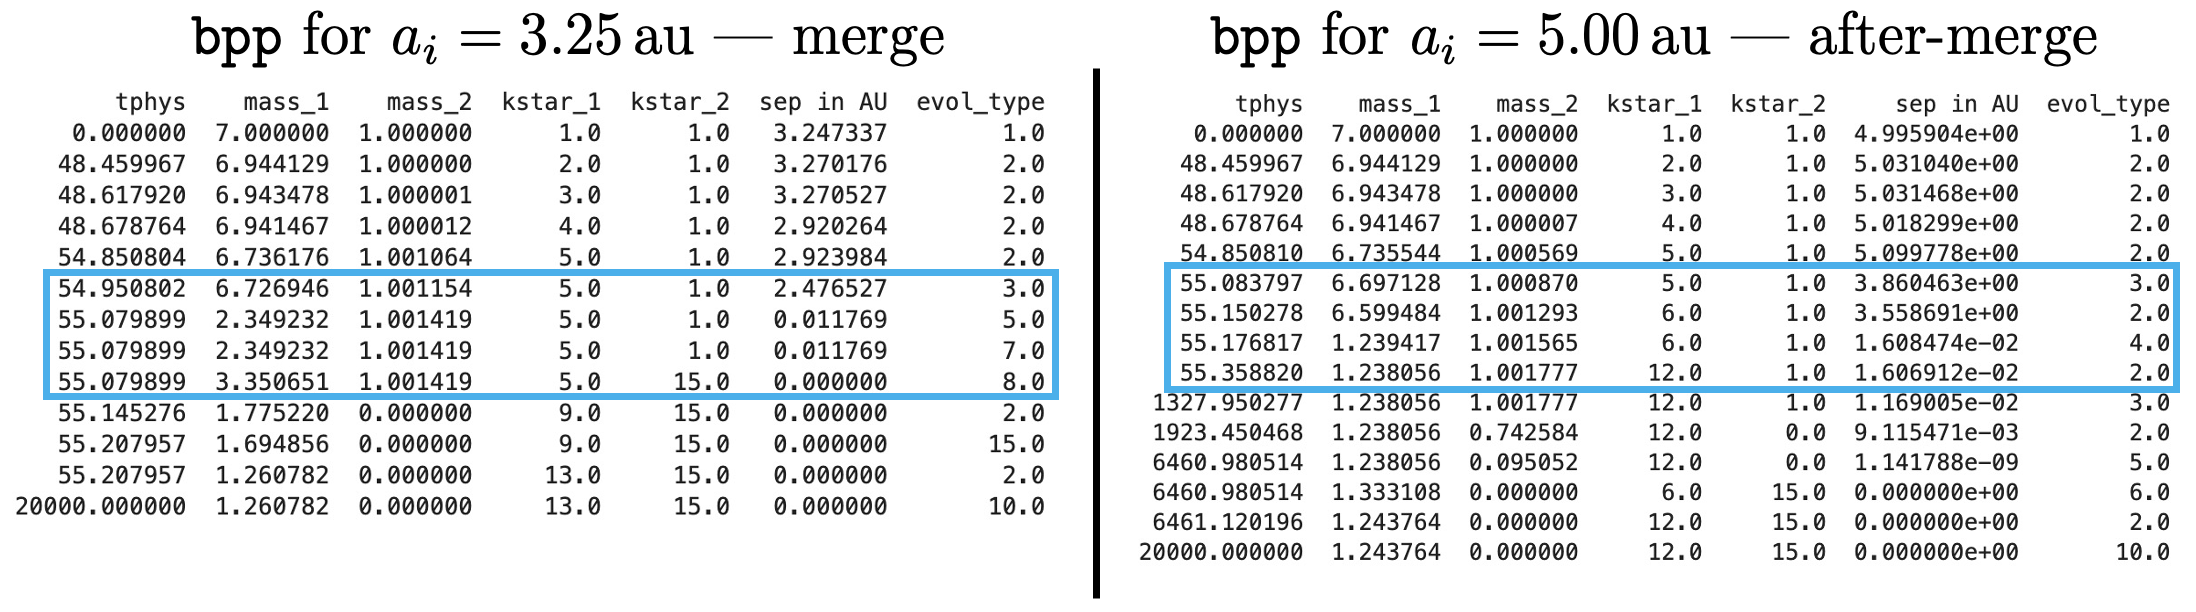
\includegraphics[width=\linewidth]{merge-after-merge.png}
    \caption{COSMIC simulation of systems $7 \Msun + 1 \Msun$ with accretion efficiency $\beta = 0$ and initial separation $3.25 \au$ and $5.00 \au$ respectively. The blue rectangle emphasizes the differences of two evolution process, which also represents the typical difference between \textbf{merge} and \textbf{after-merge} systems.}
    \label{merge-after-merge}
\end{figure}

A typical \textbf{merge} and an \textbf{after-merge} system are presented in Figure \ref{merge-after-merge}. Notice that for the merge systems, the two stars come in contact and a common envelope process follows, similar to \textbf{spike} systems. Compared to the \textbf{spike} systems, we notice that the separation of the binary at the start of the common envelope is smaller in \textbf{merge} systems than in \textbf{spike} systems. This qualitatively explains the reason for the merging — the orbit does not have enough energy to eject the common envelope and two star merges. In contrast, the \textbf{after-merge} systems possesses more energy than the \textbf{merge} systems due to their larger initial separation. Hence, they either survives the common envelope or do not come into contact at all. This explains why desired WD+MS systems form again as the initial separation $a_i$ increases.

This concludes our qualitative analysis on the evolution results of $7\Msun + 1\Msun$ through stable mass transfer. Again, as shown in Figure \ref{stable_hi}, for stable mass transfer, the observed minimum separation of wide post-mass transfer WD+MS systems $0.15 \au$ can only be achieved in the \textbf{spike} region. That is, in our results, all wide post-mass transfer systems are due to the strong wind mass loss from the primary that widens the orbit significantly.

Similarly, in \cite{yamaguchi_lo}, the author listed several arguments against the formation of wide post-mass transfer binaries through stable mass transfer. As shown in Figure \ref{theory-observed}, the observed wide post-mass transfer WD+MS binaries do not match the theoretical $M_{\mathrm{WD}} - P_{\mathrm{orb}}$ relation calculated in \cite{rappaport1995relation}, where the grey region is set to be a factor of 2.5 away from the calculated line.

\begin{figure}
    \centering
    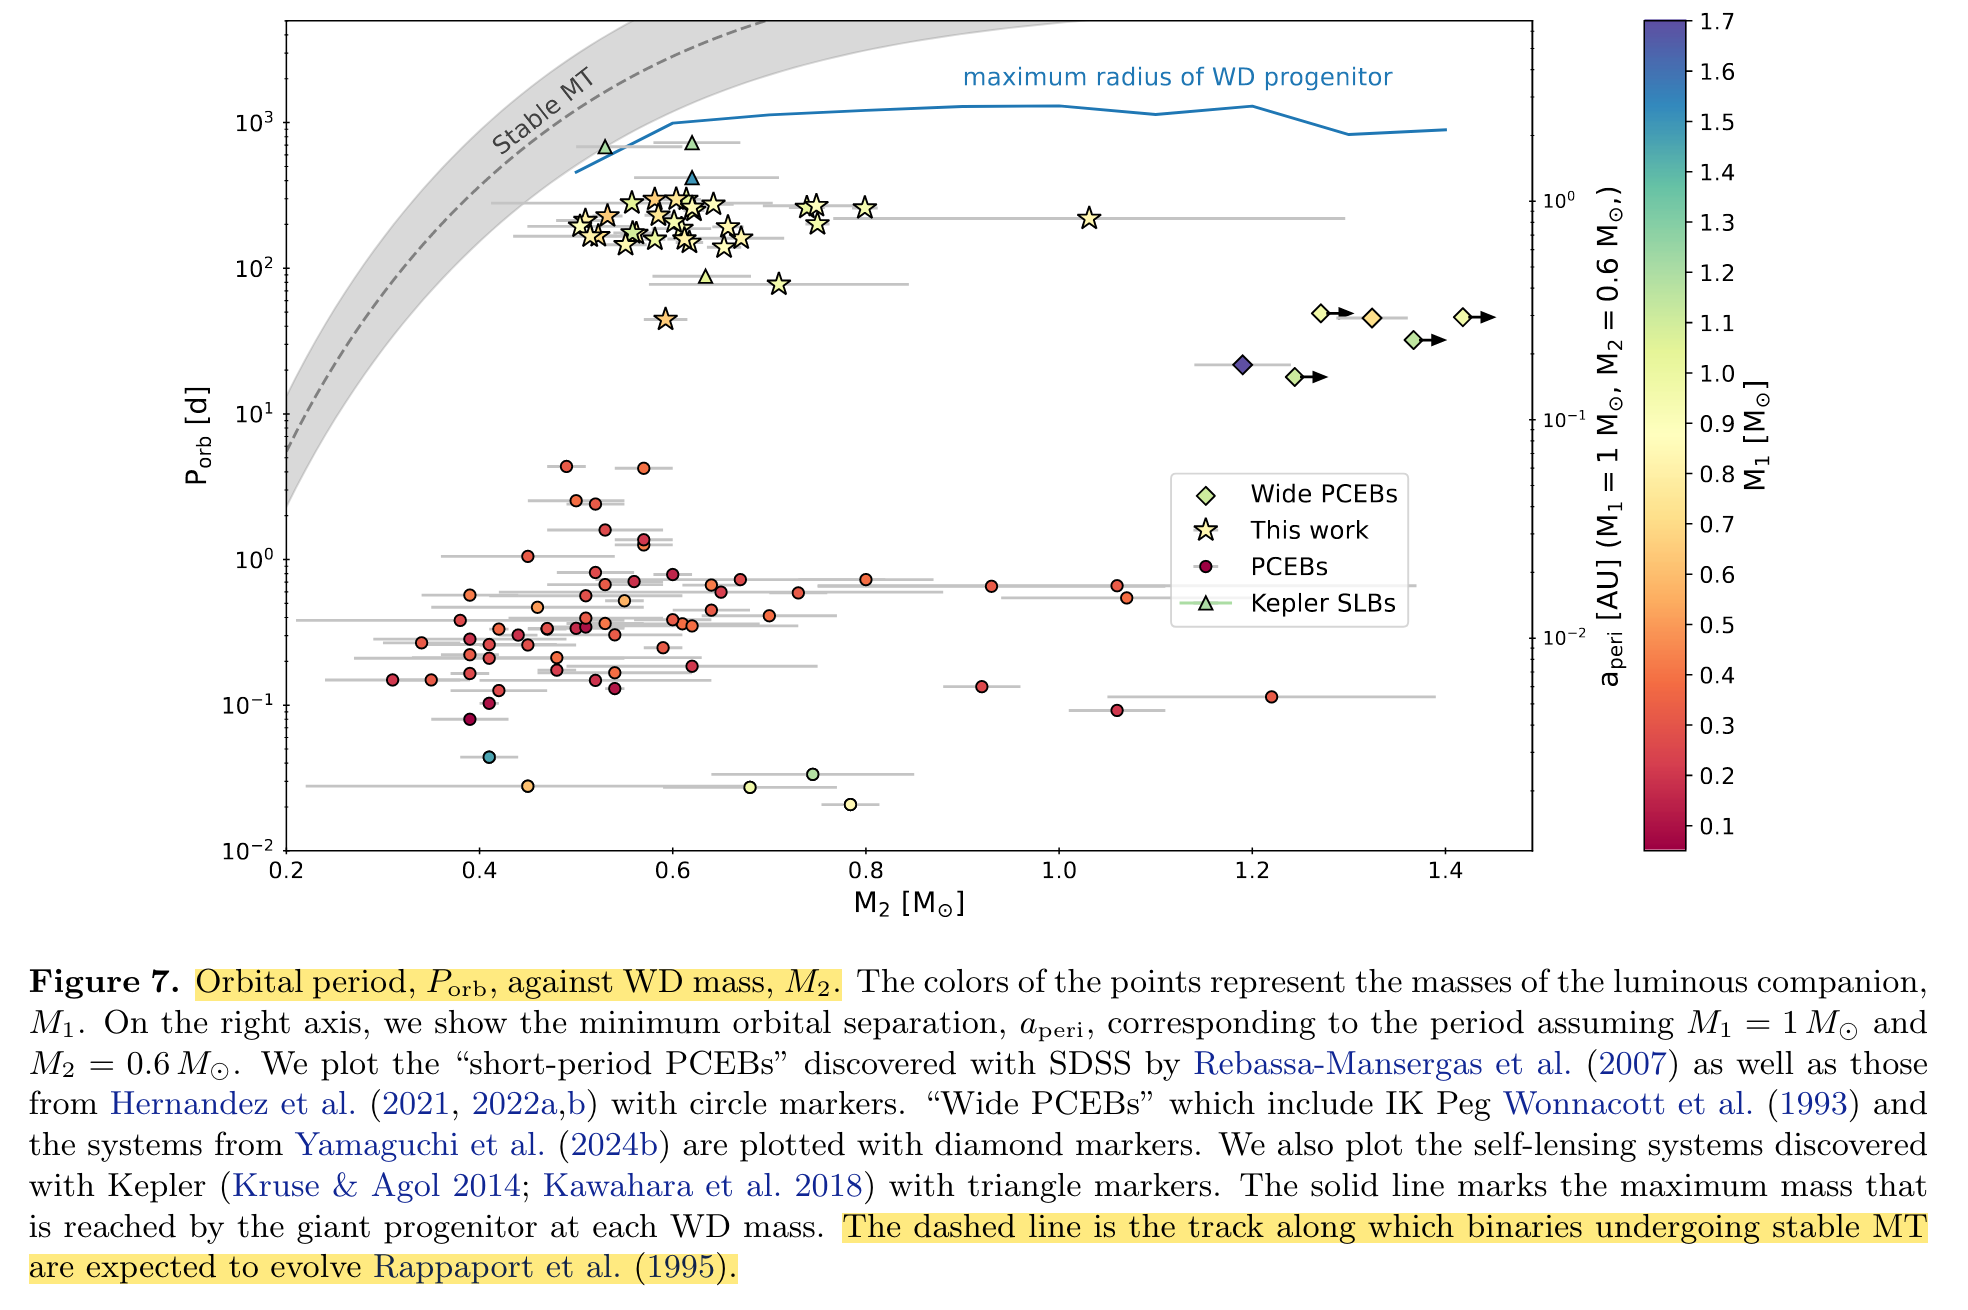
\includegraphics[width=\linewidth]{theory-observed.png}
    \caption{$M_{\mathrm{WD}} - P_{\mathrm{orb}}$ relation of observed wide post-mass transfer binaries. Binaries going through stable mass transfer is expected to fall in the grey region, as calculated in \cite{rappaport1995relation}.}
    \label{theory-observed}
\end{figure}

\section{Population Simulation}
After investigating how the final separation depends on various parameters in individual binary star systems, we now shift our focus onto the distribution of final orbital period in a population of binaries (or equivalently final separation since $\Porb^2 \sim a^3$).

\subsection{Methods}

First of all, we sample the binary population using the independent sampler in COSMIC. We set the primary mass model to \verb|korupa01|, eccentricity model to \verb|uniform|, and orbital period model, together with the binary fraction model to \verb|moe19|. We sample a total number of about 10000 binaries with solar metallicity. The distribution of primary mass and the orbital period in the sampled population is shown in the Figure \ref{sample-distribution}.

\begin{figure}
	\centering
	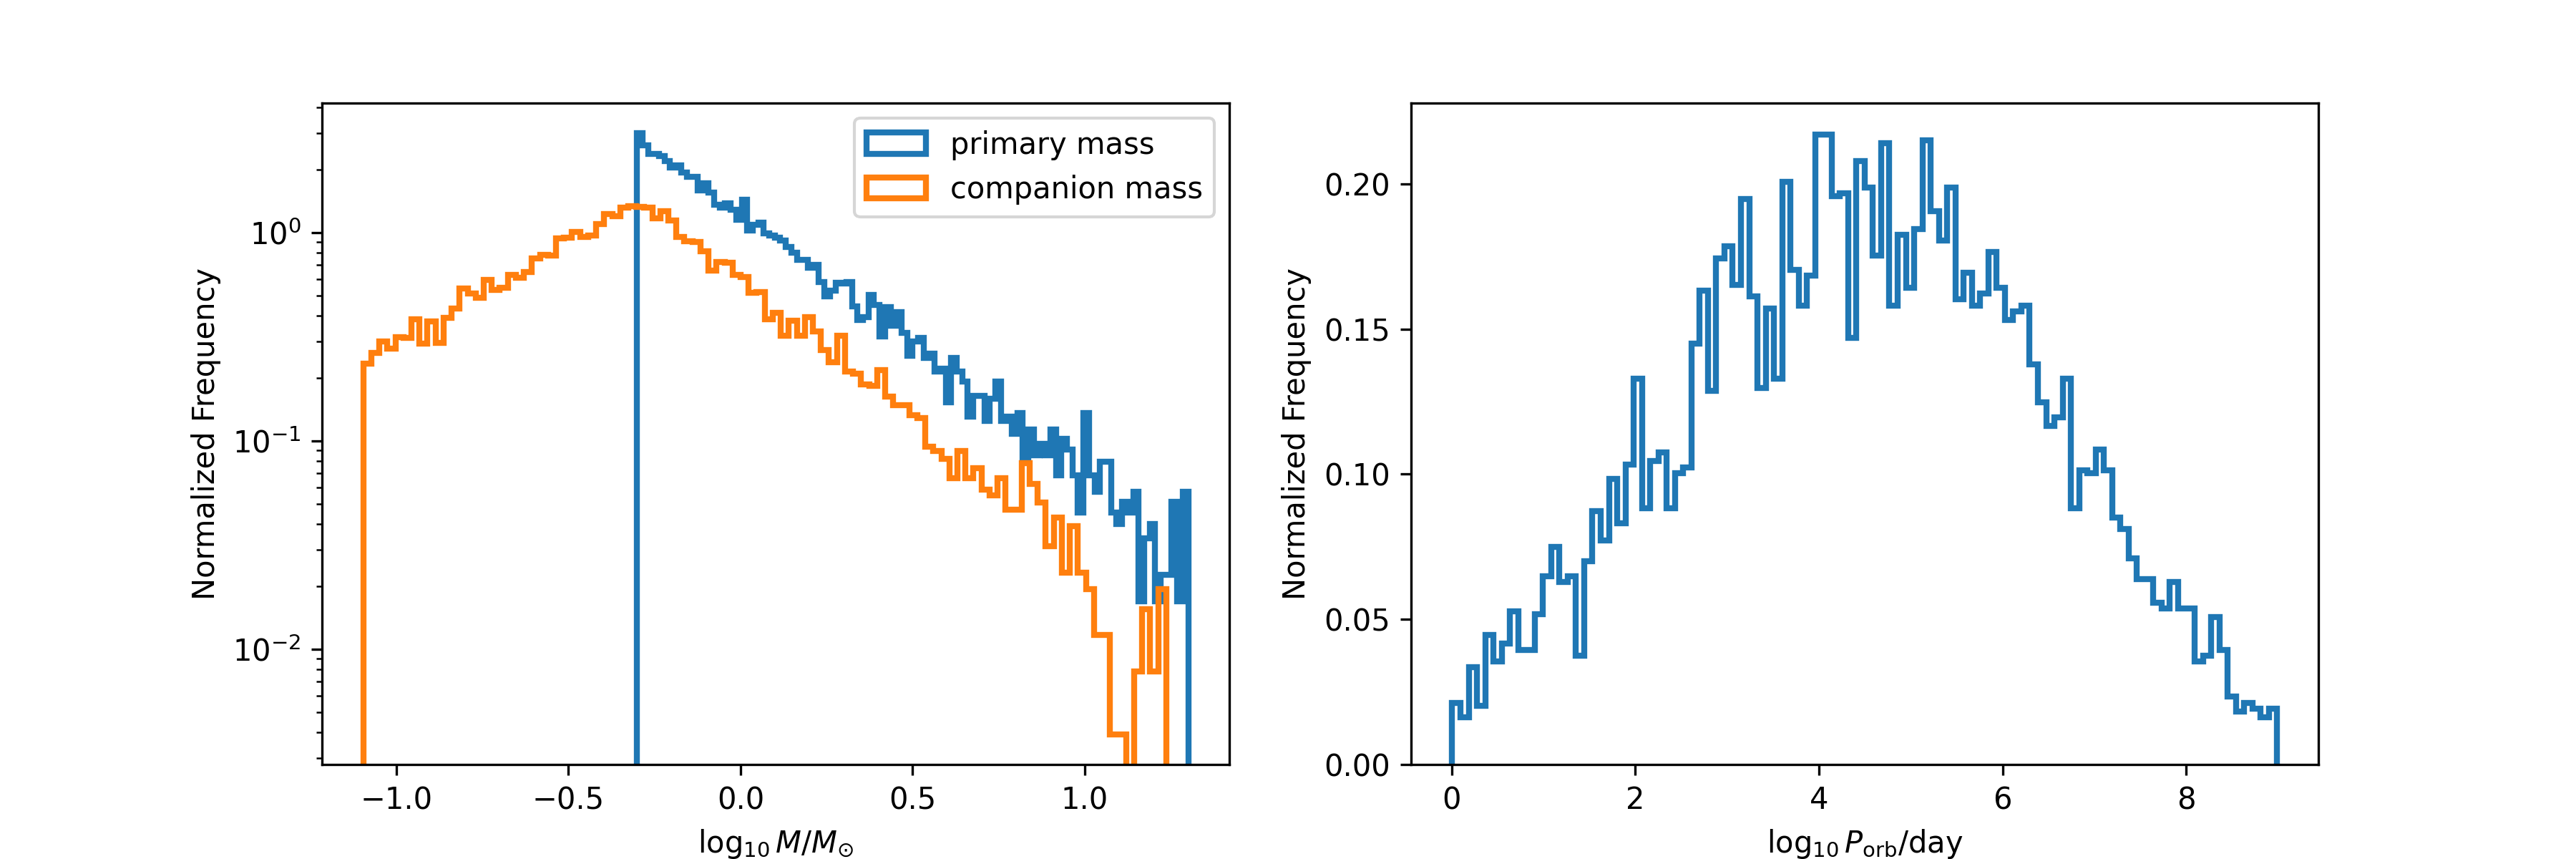
\includegraphics[width=\linewidth]{sample-distribution.png}
	\caption{The distribution of primary mass, companion mass, and orbital period in the sampled population using independent sampler. \emph{Left:} Distribution of primary mass and companion mass in log scale. \emph{Right:} Distribution of orbital period $\Porb$ in log scale.}
	\label{sample-distribution}
\end{figure}

Now to investigate how the final white dwarf mass and orbital period depends on \verb|lambdaf|, we simulation the sampled population with five different \verb|lambdaf| values, $-5$, $-15$, $-25$, $-35$, and $-45$, which corresponds to $\lambda = 5$, $15$, $25$, $35$ and $45$ in Equation \ref{ebind}. After that, for each binary star system in the population, we select the moment when CE is finished and when the system is a WD+MS one to record the white dwarf mass $\MWD$ and final orbital period $P_{\mathrm{orb}, f}$. We also select the moment when the first RLOF started to record the initial orbital separation $P_{\mathrm{orb}, i}$. This will later on help us compare the difference and how much the orbit widens.

\subsection{Results}

\begin{figure}
	\centering
	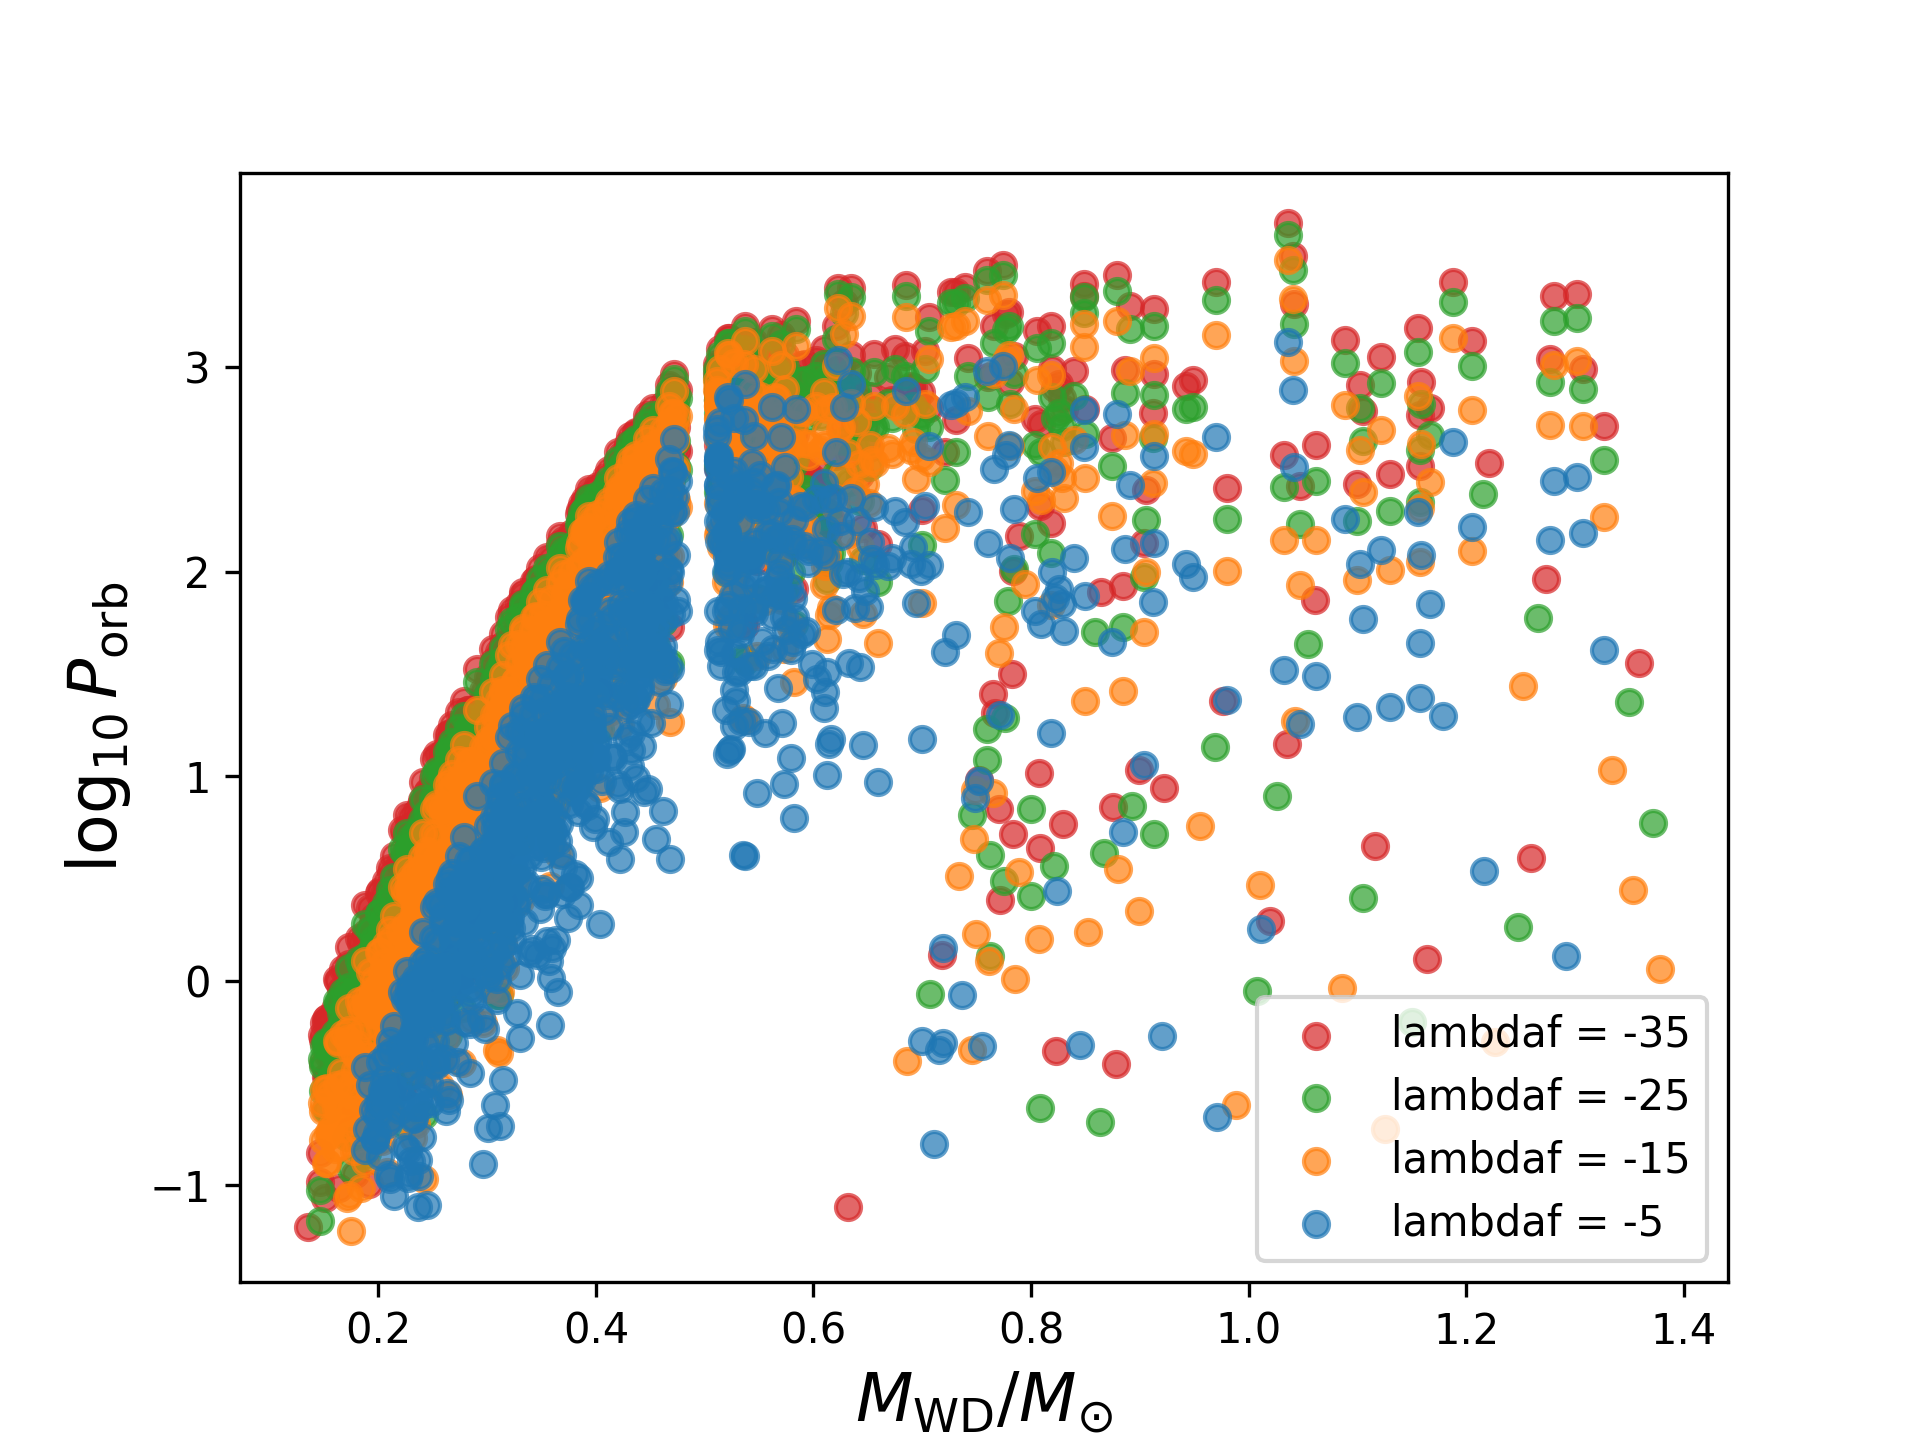
\includegraphics[width=0.5\linewidth]{Mwd-P scatter.png}
	\caption{Scatter plot of white dwarf mass $\MWD$ and final orbital period after common envelope in log scale $\log_{10}\Porb$. Different colors indicates results for different $\lambda$ values. For each different $\lambda$ value the same initial population is used.}
	\label{Mwd-P-scatter}
\end{figure}

To show how the change in $\lambda$ affects the final orbital period, a scatter plot presenting the correlation of final orbital period $\Porb$ and white dwarf mass $\MWD$ is presented in Figure \ref{Mwd-P-scatter}. We can see from the figure that when $\lambda$ increases, the final orbital period also increases. This is obvious for low $\MWD$. This correlation is expected since for larger $\lambda$, less energy is require to unbind the common envelope.

\begin{figure}
	\centering
	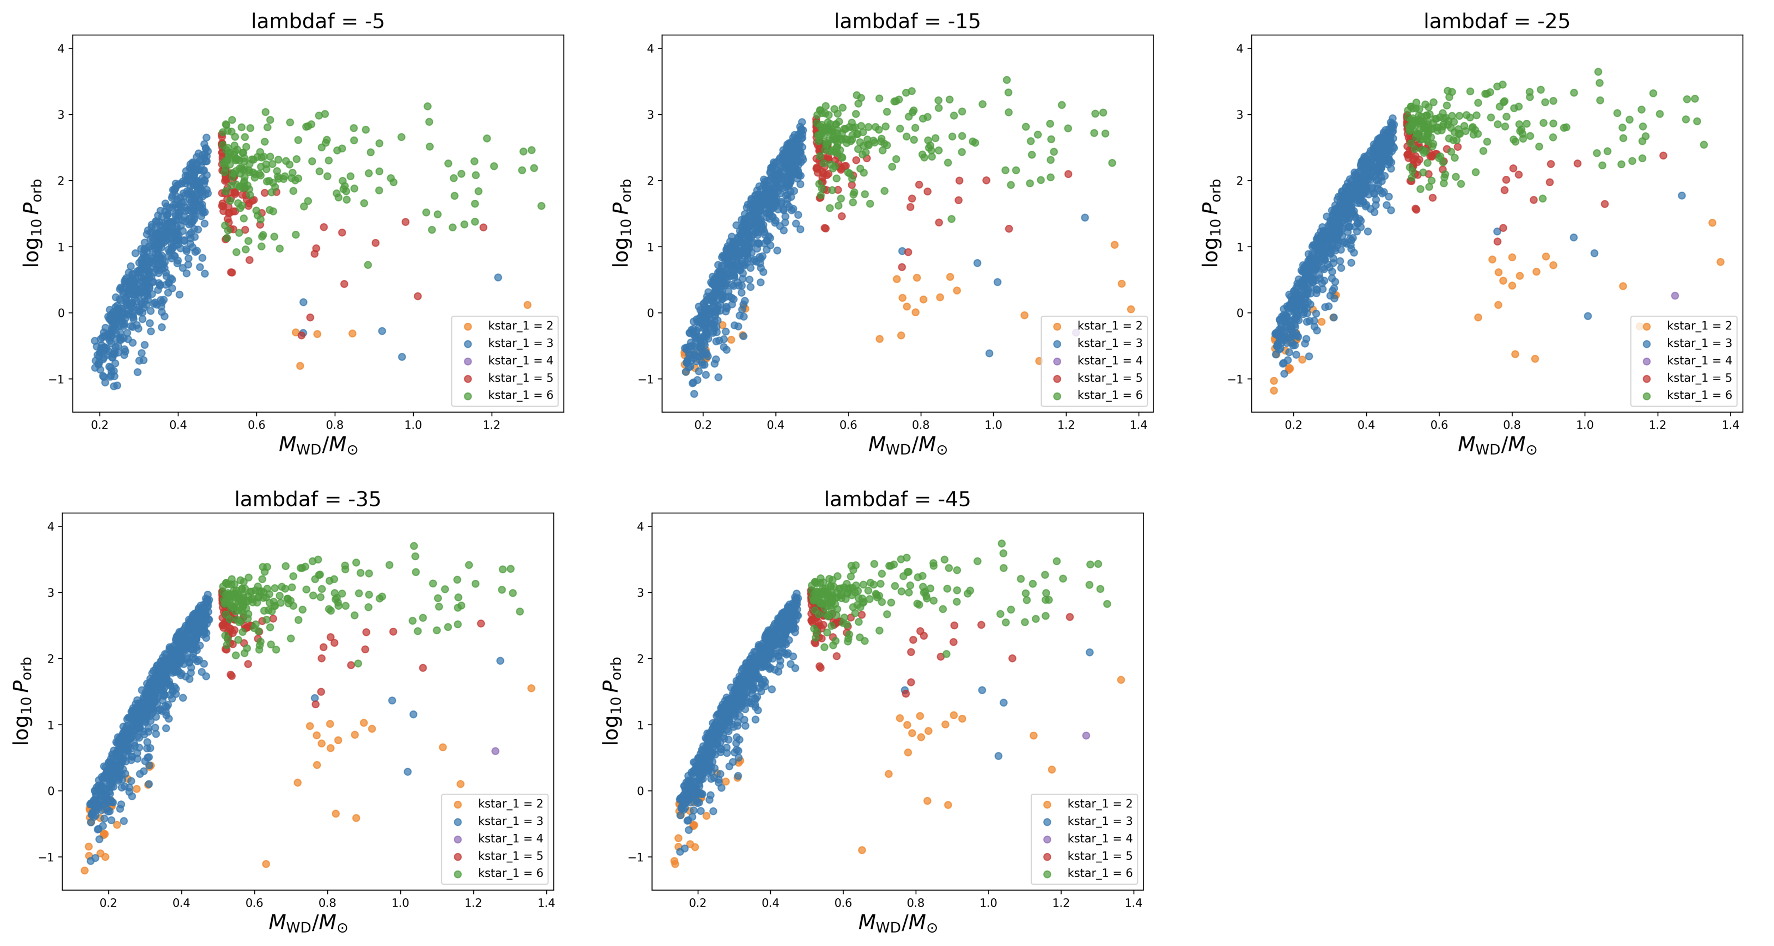
\includegraphics[width=\linewidth]{kstar-map-rearr.png}
	\caption{Each panel: for this $\lambda$ value, scatter plot of white dwarf mass $\MWD$ and final orbital period after common envelope in log scale $\log_{10}\Porb$. Different colors represent different kstar type of the primary at the start of mass transfer.}
	\label{kstar-map}
\end{figure}

To also show how the final orbital separation $\Porb$ depends on the \verb|kstar_1| type at the start of first RLOF, we plot final orbital period $\Porb$ against white dwarf mass $\MWD$ for each \verb|lambdaf| separately, and use different color to distinguish between different \verb|kstar_1| type at the start of mass transfer. The plot is shown in Figure \ref{kstar-map}. We can see that if the star is at later stages of evolution (\verb|kstar| large) when mass transfer starts, then the resulting white dwarf mass $\MWD$ and orbital period $\Porb$ is also larger. Notice that few systems start the mass transfer at \verb|kstar_1 = 2| (Hertzsprung Gap) and \verb|kstar_1 = 4| (Core Helium Burning). This is because stars crosses Hertzsprung gap in a short timescale, leaving little time for interaction. Also, stellar radius is small when going through Core Helium Burning, reducing the possibility of interactions that starts when \verb|kstar_1 = 4|.

To visualize the difference in final orbital period $\Porb$, and how they corresponds to different \verb|kstar_1| type at the start of RLOF, we create scatter plot in Figure \ref{dif-kstar map} of the difference in orbital period $\Delta P = P_{\mathrm{orb}}^{\lambda = 35} - P_{\mathrm{orb}}^{\lambda = 5}$ against the white dwarf mass $\MWD$.

\begin{figure}
	\centering
	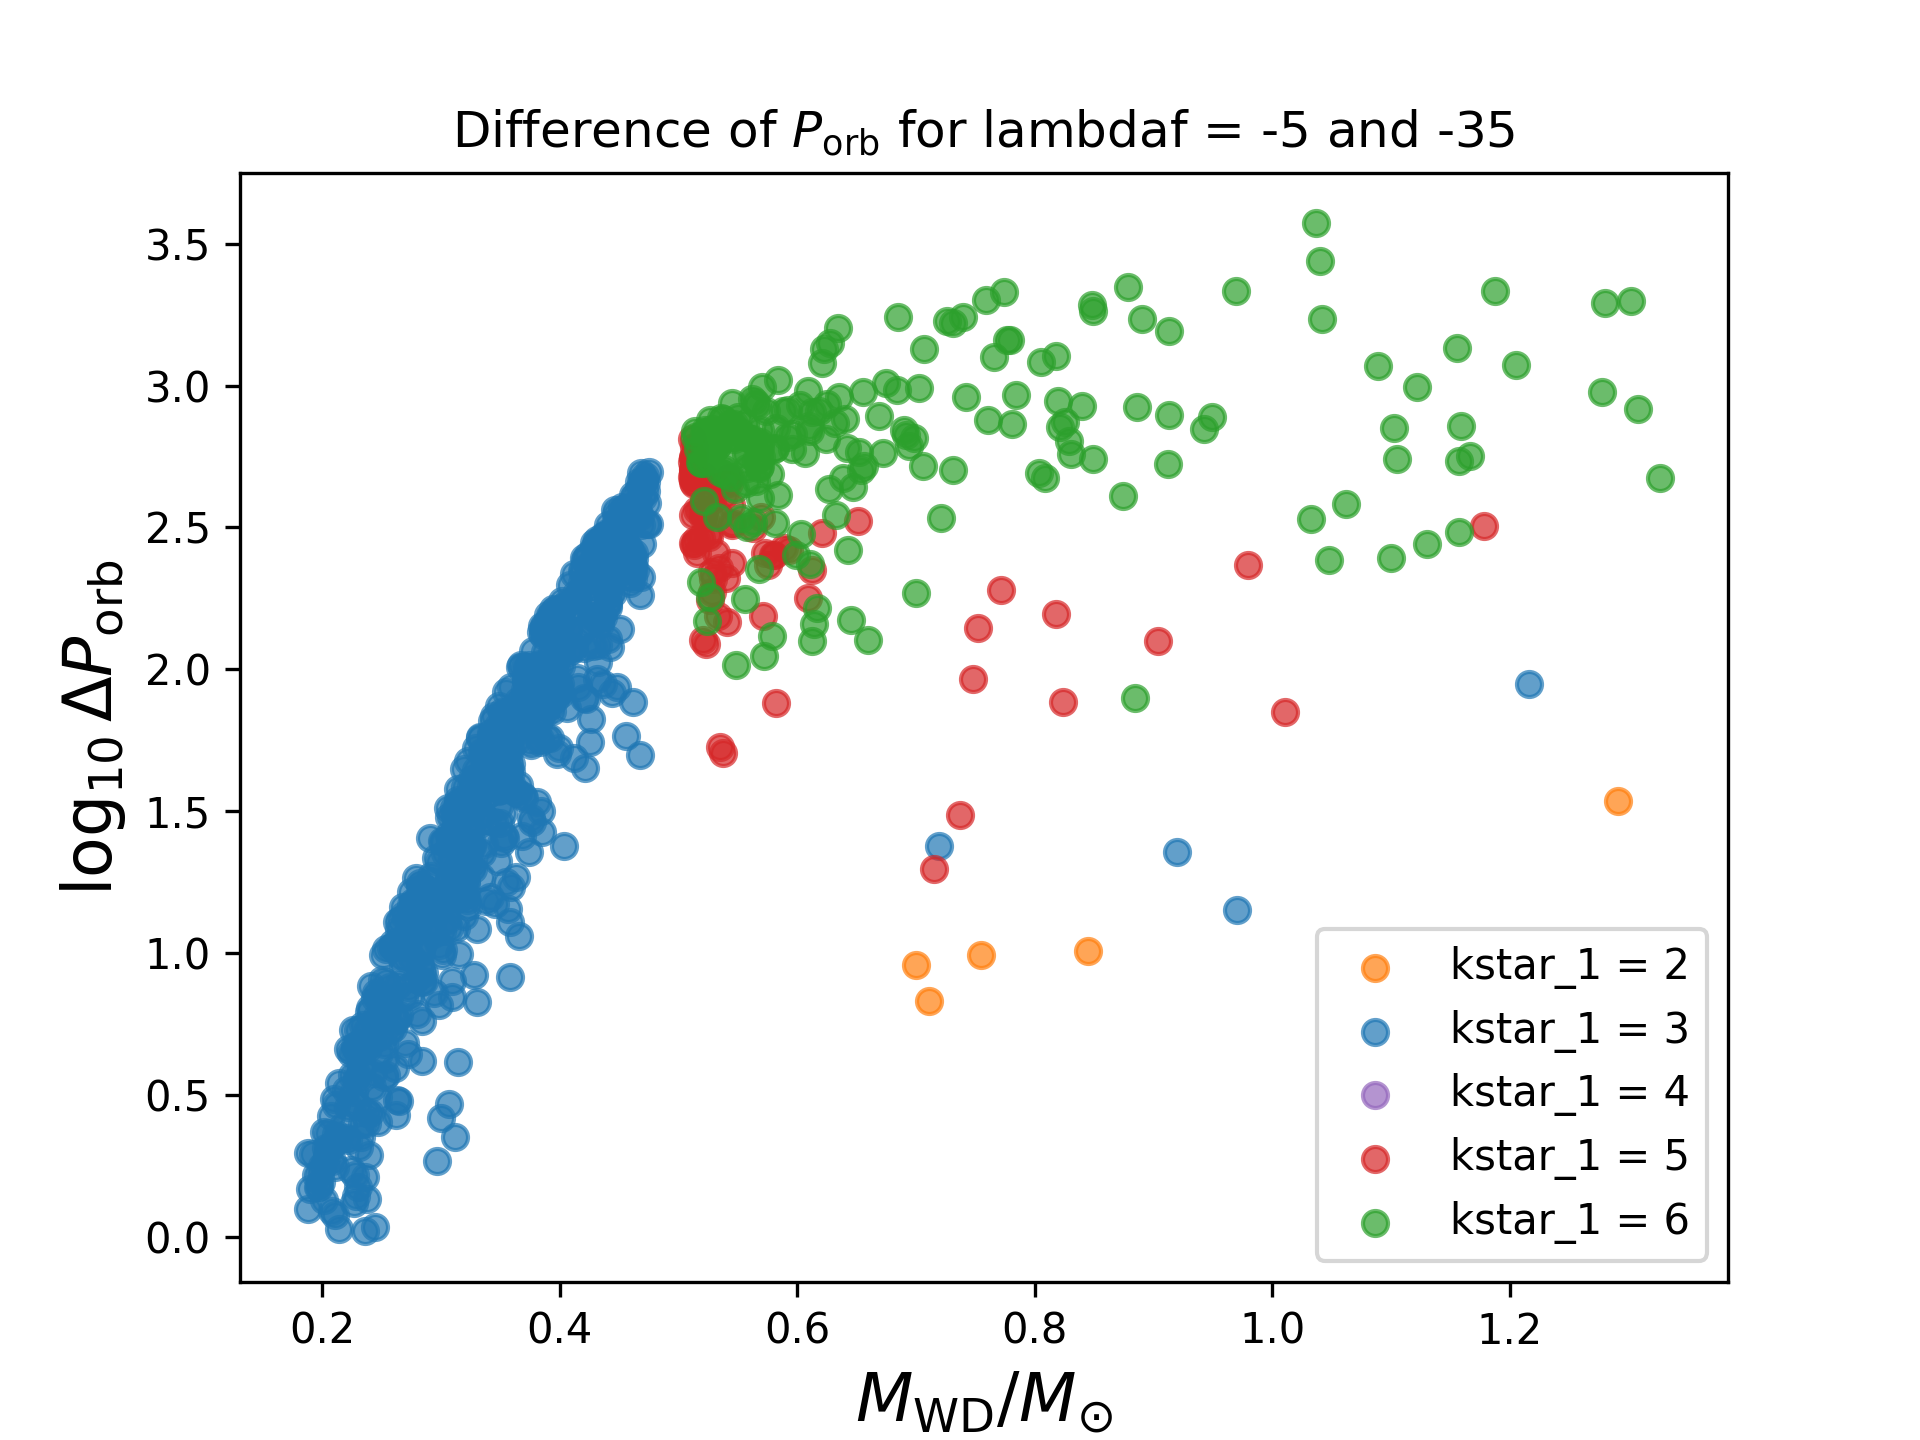
\includegraphics[width=0.5\linewidth]{dif-kstar map.png}
	\caption{Scatter plot of difference in orbital period $\Delta P = P_{\mathrm{orb}}^{\lambda = 35} - P_{\mathrm{orb}}^{\lambda = 5}$ against the white dwarf mass $\MWD$. Different colors indicates different kstar type of the primary at the start of mass transfer.}
	\label{dif-kstar map}
\end{figure}

From Figure \ref{dif-kstar map}, we can see that for large \verb|kstar_1| type at the start of RLOF, $\Delta P = P_{\mathrm{orb}}^{\lambda = 35} - P_{\mathrm{orb}}^{\lambda = 5}$ is also larger. To explain this, we plot the how final white dwarf mass $\MWD$, difference in final orbital period $\Delta \Porb$, and orbital period before mass transfer $P_{\mathrm{orb}, i}$ related to each other in Figure \ref{dif-kstar-exp}. We see that the larger initial orbital period $P_{\mathrm{orb}, i}$, the more significant effect does $\lambda$ have on the final orbital period. This is not unexpected since during mass transfer, the separation changes as $\dot{a} / a = \text{const}$. Hence $\dot{\Porb} / \Porb = \text{const}$. Therefore, the larger the initial orbital period, the larger it changes, and thus the larger effect does $\lambda$ have.

\begin{figure}
	\centering
	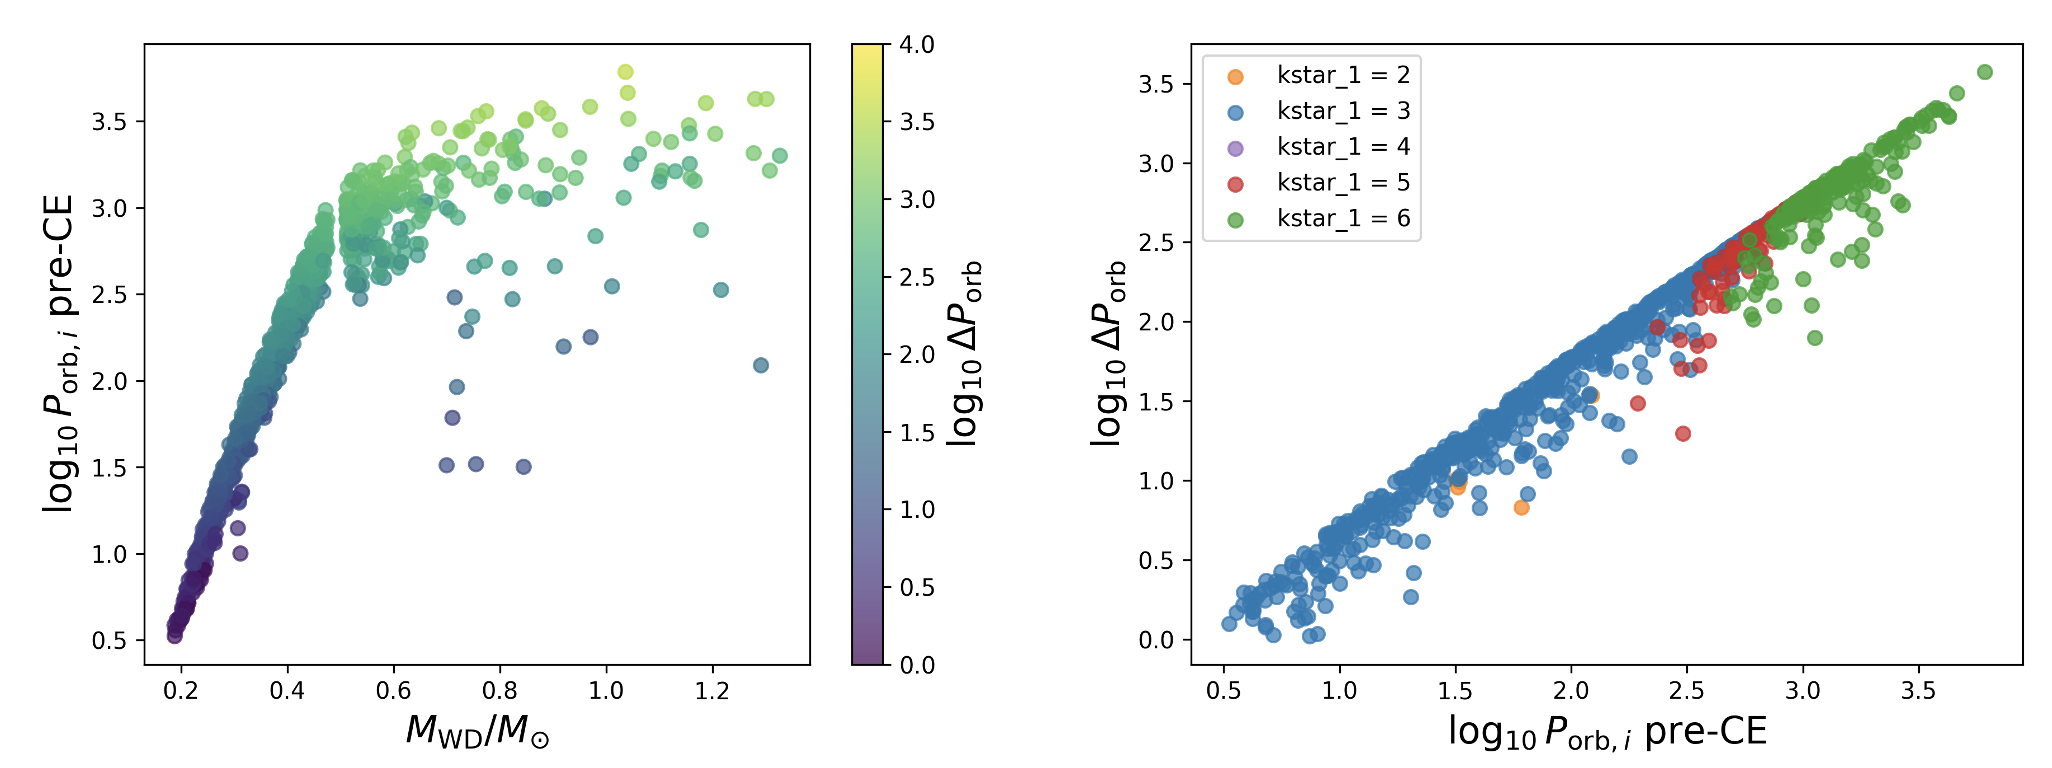
\includegraphics[width=\linewidth]{dif-kstar two plot.png}
	\caption{Left panel: scatter plot of initial orbital period at the start of RLOF $P_{\mathrm{orb}, i}$ against the final white dwarf mass $\MWD$. The color of the dots indicates how the final orbital period $P_{\mathrm{orb}, f}$ changes with respect to $\lambda=35$ and $\lambda=5$. That is, the color indicates the magnitude of $\Delta P = P_{\mathrm{orb}}^{\lambda = 35} - P_{\mathrm{orb}}^{\lambda = 5}$. Right panel: scatter plot of $\log_{10} \Delta \Porb$ against the initial orbital period in log scale $\log_{10} P_{\mathrm{orb}, i}$ at the start of RLOF. Different colors indicates different kstar type of the primary at the start of RLOF.}
	\label{dif-kstar-exp}
\end{figure}

\bibliographystyle{apalike}
\bibliography{reference.bib}

\end{document}
